\documentclass[a4paper,12pt,twoside]{memoir}

\setsecnumdepth{subsubsection}

% Castellano
\usepackage[spanish,es-tabla]{babel}
\selectlanguage{spanish}
\usepackage[utf8]{inputenc}
\usepackage[T1]{fontenc}
\usepackage{lmodern} % Scalable font
\usepackage{microtype}
\usepackage{placeins}
\usepackage{dirtree}
\usepackage{listings}
\usepackage[hyphens]{url}
\usepackage{booktabs}
\usepackage{tabularx}
\usepackage[open=true]{bookmark}


\usepackage{tocbasic}
\DeclareTOCStyleEntry[numwidth=3em]{tocline}{figure}% for figure entries
\DeclareTOCStyleEntry[numwidth=3em]{tocline}{table}% for table entries

\RequirePackage{booktabs}
\RequirePackage[table]{xcolor}
\RequirePackage{xtab}
\RequirePackage{multirow}

\lstset{%
	basicstyle=\small\ttfamily
}

% Links
%\usepackage[colorlinks]{hyperref}
%\hypersetup{
%	allcolors = {red},
%	breaklinks = true,
%}

% Ecuaciones
\usepackage{amsmath}
 
% Rutas de fichero / paquete
\newcommand{\ruta}[1]{{\sffamily #1}}

% Párrafos
\nonzeroparskip

% Huérfanas y viudas
\widowpenalty100000
\clubpenalty100000

% Evitar solapes en el header
\nouppercaseheads

% Imagenes
\usepackage{graphicx}
\newcommand{\imagen}[2]{
	\begin{figure}[!h]
		\centering
		\includegraphics[width=0.9\textwidth]{#1}
		\caption{#2}\label{fig:#1}
	\end{figure}
	\FloatBarrier
}

\newcommand{\imagenflotante}[2]{
	\begin{figure}%[!h]
		\centering
		\includegraphics[width=0.9\textwidth]{#1}
		\caption{#2}\label{fig:#1}
	\end{figure}
}



% El comando \figura nos permite insertar figuras comodamente, y utilizando
% siempre el mismo formato. Los parametros son:
% 1 -> Porcentaje del ancho de página que ocupará la figura (de 0 a 1)
% 2 --> Fichero de la imagen
% 3 --> Texto a pie de imagen
% 4 --> Etiqueta (label) para referencias
% 5 --> Opciones que queramos pasarle al \includegraphics
% 6 --> Opciones de posicionamiento a pasarle a \begin{figure}
\newcommand{\figuraConPosicion}[6]{%
  \setlength{\anchoFloat}{#1\textwidth}%
  \addtolength{\anchoFloat}{-4\fboxsep}%
  \setlength{\anchoFigura}{\anchoFloat}%
  \begin{figure}[#6]
    \begin{center}%
      \Ovalbox{%
        \begin{minipage}{\anchoFloat}%
          \begin{center}%
            \includegraphics[width=\anchoFigura,#5]{#2}%
            \caption{#3}%
            \label{#4}%
          \end{center}%
        \end{minipage}
      }%
    \end{center}%
  \end{figure}%
}

%
% Comando para incluir imágenes en formato apaisado (sin marco).
\newcommand{\figuraApaisadaSinMarco}[5]{%
  \begin{figure}%
    \begin{center}%
    \includegraphics[angle=90,height=#1\textheight,#5]{#2}%
    \caption{#3}%
    \label{#4}%
    \end{center}%
  \end{figure}%
}
% Para las tablas
\newcommand{\otoprule}{\midrule [\heavyrulewidth]}
%
% Nuevo comando para tablas pequeñas (menos de una página).
\newcommand{\tablaSmall}[5]{%
 \begin{table}[h]
  \begin{center}
   \rowcolors {2}{gray!35}{}
   \begin{tabularx}{\textwidth}{#2}
    \toprule
    #4
    \otoprule
    #5
    \bottomrule
   \end{tabularx}
   \caption{#1}
   \label{tabla:#3}
  \end{center}
 \end{table}
}

%
% Nuevo comando para tablas pequeñas (menos de una página).
\newcommand{\tablaSmallSinColores}[5]{%
 \begin{table}[H]
  \begin{center}
   \begin{tabular}{#2}
    \toprule
    #4
    \otoprule
    #5
    \bottomrule
   \end{tabular}
   \caption{#1}
   \label{tabla:#3}
  \end{center}
 \end{table}
}

\newcommand{\tablaApaisadaSmall}[5]{%
\begin{landscape}
  \begin{table}
   \begin{center}
    \rowcolors {2}{gray!35}{}
    \begin{tabular}{#2}
     \toprule
     #4
     \otoprule
     #5
     \bottomrule
    \end{tabular}
    \caption{#1}
    \label{tabla:#3}
   \end{center}
  \end{table}
\end{landscape}
}

%
% Nuevo comando para tablas grandes con cabecera y filas alternas coloreadas en gris.
\newcommand{\tabla}[6]{%
  \begin{center}
    \tablefirsthead{
      \toprule
      #5
      \otoprule
    }
    \tablehead{
      \multicolumn{#3}{l}{\small\sl continúa desde la página anterior}\\
      \toprule
      #5
      \otoprule
    }
    \tabletail{
      \hline
      \multicolumn{#3}{r}{\small\sl continúa en la página siguiente}\\
    }
    \tablelasttail{
      \hline
    }
    \bottomcaption{#1}
    \rowcolors {2}{gray!35}{}
    \begin{xtabular}{#2}
      #6
      \bottomrule
    \end{xtabular}
    \label{tabla:#4}
  \end{center}
}

%
% Nuevo comando para tablas grandes con cabecera.
\newcommand{\tablaSinColores}[6]{%
  \begin{center}
    \tablefirsthead{
      \toprule
      #5
      \otoprule
    }
    \tablehead{
      \multicolumn{#3}{l}{\small\sl continúa desde la página anterior}\\
      \toprule
      #5
      \otoprule
    }
    \tabletail{
      \hline
      \multicolumn{#3}{r}{\small\sl continúa en la página siguiente}\\
    }
    \tablelasttail{
      \hline
    }
    \bottomcaption{#1}
    \begin{xtabular}{#2}
      #6
      \bottomrule
    \end{xtabular}
    \label{tabla:#4}
  \end{center}
}

%
% Nuevo comando para tablas grandes sin cabecera.
\newcommand{\tablaSinCabecera}[5]{%
  \begin{center}
    \tablefirsthead{
      \toprule
    }
    \tablehead{
      \multicolumn{#3}{l}{\small\sl continúa desde la página anterior}\\
      \hline
    }
    \tabletail{
      \hline
      \multicolumn{#3}{r}{\small\sl continúa en la página siguiente}\\
    }
    \tablelasttail{
      \hline
    }
    \bottomcaption{#1}
  \begin{xtabular}{#2}
    #5
   \bottomrule
  \end{xtabular}
  \label{tabla:#4}
  \end{center}
}

\newcommand{\hrefFootnote}[2]{%
	\href{#1}{#2}\footnote{\url{#1}}
}

\newcommand{\code}[1]{\texttt{#1}}


\definecolor{cgoLight}{HTML}{EEEEEE}
\definecolor{cgoExtralight}{HTML}{FFFFFF}

%
% Nuevo comando para tablas grandes sin cabecera.
\newcommand{\tablaSinCabeceraConBandas}[5]{%
  \begin{center}
    \tablefirsthead{
      \toprule
    }
    \tablehead{
      \multicolumn{#3}{l}{\small\sl continúa desde la página anterior}\\
      \hline
    }
    \tabletail{
      \hline
      \multicolumn{#3}{r}{\small\sl continúa en la página siguiente}\\
    }
    \tablelasttail{
      \hline
    }
    \bottomcaption{#1}
    \rowcolors[]{1}{cgoExtralight}{cgoLight}

  \begin{xtabular}{#2}
    #5
   \bottomrule
  \end{xtabular}
  \label{tabla:#4}
  \end{center}
}


\graphicspath{ {./img/} }

% Capítulos
\chapterstyle{bianchi}
\newcommand{\capitulo}[2]{
	\setcounter{chapter}{#1}
	\setcounter{section}{0}
	\chapter*{#2}
	\addcontentsline{toc}{chapter}{#1. #2}
	\markboth{#2}{#2}
}

% Apéndices
\renewcommand{\appendixname}{Apéndice}
\renewcommand*\cftappendixname{\appendixname}

\newcommand{\apendice}[1]{
	%\renewcommand{\thechapter}{A}
	\chapter{#1}
}

\renewcommand*\cftappendixname{\appendixname\ }

% Formato de portada
\makeatletter
\usepackage{xcolor}
\newcommand{\tutor}[1]{\def\@tutor{#1}}
\newcommand{\cotutor}[1]{\def\@cotutor{#1}}
\newcommand{\course}[1]{\def\@course{#1}}
\definecolor{cpardoBox}{HTML}{E6E6FF}
\def\maketitle{
	\null
	\thispagestyle{empty}
	% Cabecera ----------------
	\begin{center}%
		{\noindent\LARGE Universidades de Burgos, León y Valladolid}\vspace{.5cm}%

		{\noindent\large Máster universitario}\vspace{.5cm}%

		{\noindent\LARGE \textbf{Inteligencia de Negocio y Big~Data en Entornos Seguros}}\vspace{.5cm}%
	\end{center}%

	\begin{center}%
		
\includegraphics[height=3cm]{img/escudoUBU} \hspace{1cm}
		
\includegraphics[height=3cm]{img/escudoUVA} \hspace{1cm}
		
\includegraphics[height=3cm]{img/escudoULE} \vspace{1cm}%
	\end{center}%

	\vfill
	% Título proyecto y escudo informática ----------------
	\colorbox{cpardoBox}{%
		\begin{minipage}{.9\textwidth}
			\vspace{.4cm}\large
			\begin{center}
				\textbf{Trabajo Fin de Máster}\vspace{.6cm}\\
				\textbf{\Large\@title{}}
			\end{center}
			\vspace{.2cm}
		\end{minipage}

	}%
	\vfill
	% Datos de alumno, curso y tutores ------------------
	\begin{center}%
		{%
			\noindent\Large
			Presentado por \@author{}\\
			en la Universidad de Burgos --- \@date{}\\[1em]
			Tutores: Dr. \@tutor{} y\\\hspace{3.7em}Dr. \@cotutor{}
		}%
	\end{center}%
	\null
	\cleardoublepage
}
\makeatother

\newcommand{\nombre}{Francisco Gil Rodríguez} %%% cambio de comando
\newcommand{\titulo}{Plugin Knime para conexión con Moodle}
\newcommand{\nombretutor}{José Francisco Díez Pastor}
\newcommand{\nombrecotutor}{César Ignacio García Osorio}
\newcommand{\fecha}{1 de febrero de 2024}

\setcounter{secnumdepth}{1}
\setcounter{tocdepth}{1}

% Datos de portada
\title{\titulo}
\author{\nombre}
\tutor{\nombretutor}
\cotutor{\nombrecotutor}
\date{\fecha}

\begin{document}

\maketitle

\newpage\null\thispagestyle{empty}\newpage


%%%%%%%%%%%%%%%%%%%%%%%%%%%%%%%%%%%%%%%%%%%%%%%%%%%%%%%%%%%%%%%%%%%%%%%%%%%%%%%%%%%%%%%%
\thispagestyle{empty}


\noindent
\begin{center}%
	{\noindent\Huge Universidades de Burgos, León y Valladolid}\vspace{.5cm}%

\begin{center}%
	
\includegraphics[height=3cm]{img/escudoUBU} \hspace{1cm}
	
\includegraphics[height=3cm]{img/escudoUVA} \hspace{1cm}
	
\includegraphics[height=3cm]{img/escudoULE} \vspace{1cm}%
\end{center}%

	{\noindent\Large \textbf{Máster universitario en Inteligencia de Negocio y Big~Data en Entornos Seguros}}\vspace{.5cm}%
\end{center}%



\noindent D. \nombretutor, profesor del departamento de Ingeniería Informática, área de Lenguajes y Sistemas Informáticos.

\noindent D. \nombrecotutor, profesor del departamento de Ingeniería Informática, área de Lenguajes y Sistemas Informáticos.

\noindent Exponen:

\noindent Que el alumno D. \nombre, con DNI 42183724E, ha realizado el Trabajo final de Máster en Inteligencia de Negocio y Big Data en Entornos Seguros
          titulado <<\titulo>>.

\noindent Y que dicho trabajo ha sido realizado por el alumno bajo la dirección del que suscribe, en virtud de lo cual se autoriza su presentación y defensa.

\begin{center} %\large
En Burgos, {\large \fecha}
\end{center}

\vfill\vfill\vfill

% Author and supervisor
\begin{minipage}{0.45\textwidth}
\begin{flushleft} %\large
Vº. Bº. del Tutor:\\[2cm]
D. \nombretutor
\end{flushleft}
\end{minipage}
\hfill
\begin{minipage}{0.45\textwidth}
\begin{flushleft} %\large
Vº. Bº. del Tutor:\\[2cm]
D. \nombrecotutor
\end{flushleft}
\end{minipage}
\hfill

\vfill


\newpage\null\thispagestyle{empty}\newpage



\frontmatter

% Abstract en castellano
\renewcommand*\abstractname{Resumen}
\begin{abstract}

KNIME es una plataforma de código abierto orientada al análisis de datos que permite, a través de una interfaz intuitiva y visual, 
crear análisis complejos y flujos de trabajo mediante componentes especializados en diferentes áreas como la minería de datos, 
el aprendizaje automático o la visualización de datos. Moodle es una plataforma de aprendizaje (Learning Management System) ampliamente 
utilizada por instituciones educativas de todo el mundo. En este trabajo se han desarrollado nuevos componentes de KNIME que permiten la 
integración en flujos de trabajo de KNIME de los datos que Moodle va registrando durante la ejecución de una acción formativa. 
Con un enfoque orientado al rol de profesor, se pretende que cualquier usuario con este rol dentro de una 
plataforma Moodle, pueda realizar estudios externos sobre los datos de las acciones formativas a las que tiene acceso. 
Adicionalmente se ha implementado un flujo de trabajo en KNIME sobre datos reales extraidos de Moodle, analizando diferentes 
técnicas de aprendizaje automático supervisado. 

\end{abstract}

\renewcommand*\abstractname{Descriptores}
\begin{abstract}
Moodle, Knime, ETL, aprendizaje automático, aprendizaje supervisado, Java
\end{abstract}

\clearpage

% Abstract en inglés
\renewcommand*\abstractname{Abstract}
\begin{abstract}
  KNIME is an open source platform oriented to data analysis that allows, through an intuitive and visual interface, the creation of 
  complex analysis and workflows through specialized components in different areas such as data mining, machine learning or data visualization. 
  Moodle is a learning platform (Learning Management System) widely used by educational institutions around the world. 
  In this work we have developed new Knime components that allow the integration of the data recorded by Moodle during the execution of
   a training action into KNIME workflows. With an approach oriented to the role of teacher, it is intended that any user with this 
   role within a Moodle platform, can perform external studies on the data of the training actions to which they have access. 
   In addition, a workflow have been implemented in KNIME on real data extracted from Moodle, analyzing different supervised machine
    learning techniques.
\end{abstract}

\renewcommand*\abstractname{Keywords}
\begin{abstract}
  Moodle, Knime, ETL, machine learning, supervised learning, Java

\end{abstract}

\clearpage


% Indices
\tableofcontents

\clearpage

\listoffigures

\clearpage

\listoftables
\clearpage

\mainmatter

\addcontentsline{toc}{part}{Memoria}
\part*{Memoria}

\capitulo{1}{Introducción}

Descripción del contenido del trabajo y del estrucutra de la memoria y del resto de materiales entregados.

\capitulo{2}{Objetivos del proyecto}
En este apartado se exponen los objetivos del proyecto, diferenciados entre objetivos generales, técnicos y personales. 

\section{Objetivos generales}

\begin{itemize}
	\item Desarrollar un plugin de KNIME que permita importar datos desde una plataforma 
	de teleformación Moodle, para su tratamiento posterior dentro de flujos de trabajo de KNIME.
	\item Facilitar la incorporación en KNIME de datos de cursos de cualquier plataforma Moodle, 
	sin necesidad de realizar ajustes personalizados dentro de la plataforma de formación. 
    \item Orientar la solución al perfil de profesor, de forma que cualquier usuario con este
	 perfil pueda realizar estudios desde KNIME de los datos relativos a sus cursos. 
    \item Implementar un ejemplo práctico utilizando el plugin de KNIME desarrollado en un
	 flujo de trabajo relacionado con aprendizaje supervisado.
\end{itemize}

\section{Objetivos técnicos}

\begin{itemize}
	\item Desarrollar un plugin para KNIME en lenguaje de programación Java. 
	\item Explorar la arquitectura de KNIME para elegir el tipo de componentes a desarrollar que mejor se adapten a la solución requerida.
	\item Conocer a fondo la metodología de programación en KNIME mediante el estudio de la documentación existente y la inspección de \english{plugins} de KNIME similares.
	\item Explorar los nodos y \english{workflows} de KNIME disponibles en el ámbito del aprendizaje supervisado.
\end{itemize}

\section{Objetivos personales}

\begin{itemize}
	\item Aplicar los conocimientos adquiridos dentro del máster en al ámbito educativo y más específicamente en el de la formación online. 
	\item Conocer más a fondo las herramientas que, como KNIME, permiten el análisis de datos desde la interfaz de usuario, tanto a nivel de usuario como a nivel de desarrollador. 
    \item Contribuir a la mejora de la formación online al facilitar que los profesores puedan realizar análisis sobre sus cursos sin conocimientos de programación. 
\end{itemize}

\capitulo{3}{Conceptos teóricos}

\section{KNIME}

KNIME es un software de código abierto orientado a la ciencia de datos. Puede ser descargado y utilizado gratuitamente bajo los términos de la Licencia Pública General de GNU versión 3 (GPLv3). A través de una interfaz gráfica intuitiva, 
permite crear flujos de trabajo de análisis de datos y minería de datos. KNIME fue desarrollado en la Universidad de 
Konstanz (Alemania) en 2004, y su nombre proviene de su denominación en inglés <<\english{Konstanz Information Miner}>>\cite{BCDG+07} \cite{knime-whitepaper}. 
\

\begin{figure}[!h]
	\centering
	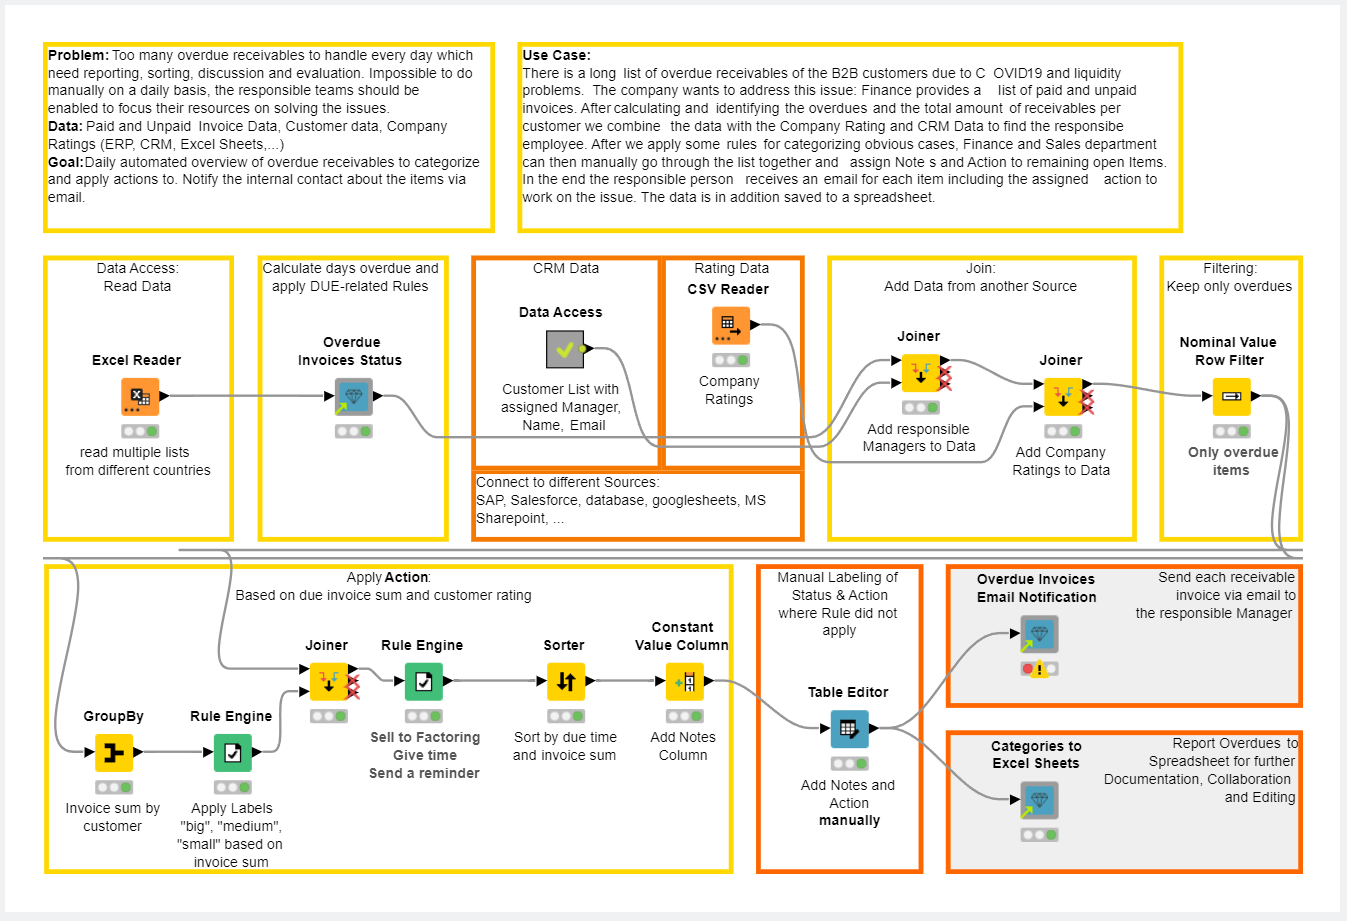
\includegraphics[width=1\textwidth]{img/3_ejemplo_workflow_knime.png}
	\caption{Ejemplo de Workflow en KNIME.}
	\label{fig:ejemploworkflow}
\end{figure}
\FloatBarrier

KNIME está concebido como una herramienta gráfica y dispone de una serie de nodos, que encapsulan distintos tipos de
 algoritmos, y flechas, que representan flujos de datos, que se despliegan y combinan de manera gráfica e interactiva.
\

KNIME cuenta con un \href{https://hub.knime.com/}{repositorio abierto} desde donde se pueden descargar nodos, \english{workflows}, componentes y extensiones. 
\

KNIME incluye más de 2000 nodos nativos, que puede extenderse con otros más de 4500 nodos disponibles en el \english{hub} 
de la comunidad. Cubre prácticamente todos los aspectos de la ciencia de datos, desde recopilar y manipular 
datos hasta darles sentido con técnicas sofisticadas de modelado y visualización.
\

El carácter abierto de la herramienta hace posible su extensión mediante la creación de nuevos nodos que 
implementen algoritmos a la medida del usuario. Además, existe la posibilidad de utilizar llamadas directas 
a Weka o de incorporar de manera sencilla código desarrollado en R o Python.
\

Además de la versión \english{Community}, que es libre y gratuita, KNIME ofrece soluciones de pago para empresas, como \english{KNIME Server} 
y \english{KNIME Business Hub}. Estas soluciones se pueden instalar en los servidores del cliente y están diseñadas para la 
colaboración en equipo, la automatización, la gestión y el despliegue de flujos de trabajo. En este proyecto nos centraremos únicamente
en la versión \english{Community}. 
\

En la arquitectura de KNIME se compone principalmente de los siguientes elementos: 

\begin{itemize}
	\item \textbf{Nodos}. Un nodo representa una función específica que se aplica a los datos. Los nodos realizan operaciones específicas, 
	 como lectura de datos, preprocesamiento, análisis, visualización o exportación de datos.
	\item \textbf{Puertos}. Los puertos son las conexiones de entrada y salida que los nodos pueden tener para conectarse y 
	 comunicarse entre ellos. 
	\item \textbf{Workflows}. Un \english{workflow} o flujo de trabajo es una representación visual de un conjunto de operaciones que se realiza 
	mediante nodos interconectados. 
	\item \textbf{Componentes}. Los componentes son nodos que contienen un subflujo de trabajo, lo que nos permite encapsular
	funcionalidad para reutilizar en diferentes flujos de trabajo. Pueden tener su propio cuadro de diálogo de configuración, lo que nos permite 
	ajustar la funcionalidad sin necesidad de modificar los componentes que contiene. 
	\item \textbf{Metanodos}. Los metanodos se utilizan para simplificar los flujos de trabajo. Se trata de seleccionar una parte del flujo, 
	compuesta por varios nodos y sus relaciones, y agruparlos en un nodo especial llamado metanodo, con lo que ocultamos esa parte del flujo 
	y lo simplificamos visualmente. A diferencia de los componentes, los metanodos se utilizan solo como contenedores para mejorar la visualización 
	de un flujo complejo, teniendo siempre que expandirlos para realizar modificaciones en esa parte del flujo de trabajo.
	\item \textbf{Extensiones}. Las extensiones son \english{plugins} adicionales que podemos añadir a KNIME para ampliar las funcionalidades que 
	no están incluidas en el núcleo. Generalmente las extensiones incluyen nodos agrupados dentro de una misma temática. 
\end{itemize}

En la Figura~\ref{fig:knime_elementos1} se muestra un \english{workflow} muy básico con dos nodos interconectados entre sí. El nodo 
\node{Table Creator} permite definir una tabla de datos con varias columnas y filas. Este nodo no tiene puerto de entrada. El puerto de salida 
devuelve los datos, y se conecta a un nodo de tipo \node{Sorter} a través de su puerto de entrada. Este otro nodo ordena los datos 
en función de la columna indicada en su configuración. El puerto de salida del nodo \node{Sorter} será 
una tabla similar a la definida en \node{Table Creator}, pero ordenada según lo especificado. 

\begin{figure}[!h]
	\centering
	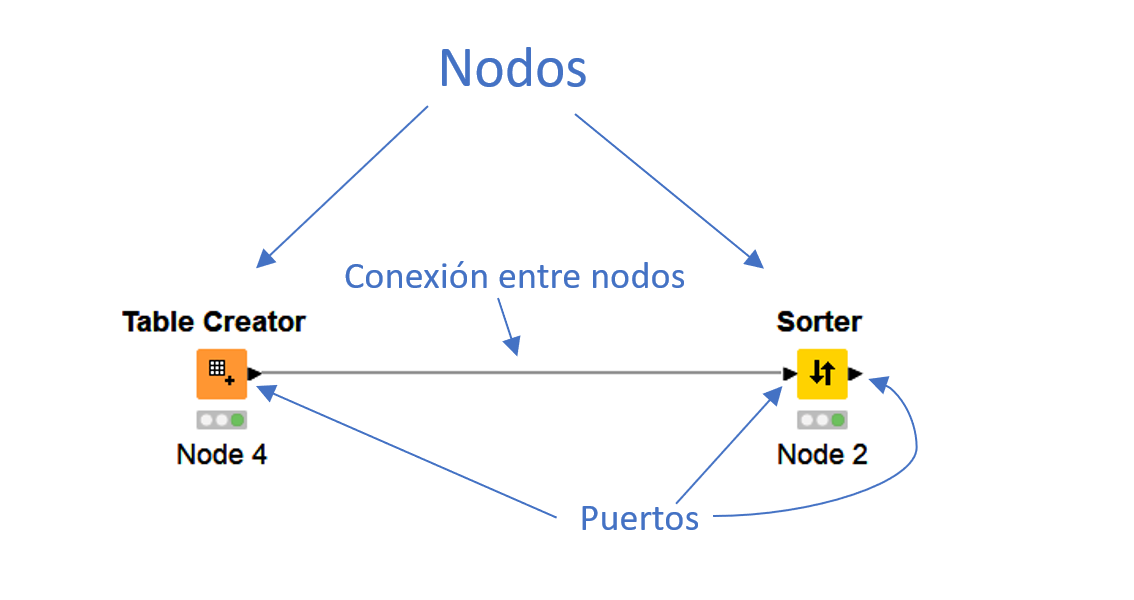
\includegraphics[width=1\textwidth]{img/knime_elementos1.png}
	\caption{\english{Workflow} de ejemplo con elementos de KNIME.}
	\label{fig:knime_elementos1}
\end{figure}
\FloatBarrier






\section{Moodle}

Moodle es una plataforma de gestión del aprendizaje (\english{LMS, Learning Management System}) de código abierto diseñada
 para crear y administrar cursos en línea. Moodle se ha convertido en una de los LMS más populares y ampliamente 
 utilizados en todo el mundo, con una importante presencia en el ámbito universitario.
\

Moodle registra en sus \english{logs} una gran variedad de información. Para este proyecto nos centraremos únicamente en 
la información que Moodle recopila relacionada con el proceso de enseñanza-aprendizaje, como puede ser: 

\begin{itemize}
  \item Registro de actividad del usuario. En estos \english{logs} se registra la actividad de los usuarios, como cuándo 
  acceden a la plataforma, cuándo ven o completan módulos de cursos, cuándo participan en foros de discusión y
   cuándo envían tareas o cuestionarios. 
  \item Registro de calificaciones en tareas y cuestionarios.
  \item Registro de mensajes y comunicación. Los \english{logs} pueden registrar la comunicación entre usuarios, 
  como mensajes internos, mensajes de foros de discusión y chat en vivo.
\end{itemize}



\section{ETL}

ETL (\english{extract, transform, load}) \cite{etl} es un proceso de tres fases en el que los datos se extraen, se transforman y se cargan en un 
contenedor de datos de salida. Los datos pueden obtenerse de una o varias fuentes y enviarse a uno o varios destinos.

\begin{itemize}
	\item \textbf{Extracción}. En esta primera fase se extraen los datos en bruto de diferentes fuentes. En este proyecto los datos 
    provienen principalmente de Moodle aunque son extraídos usando diferentes técnicas (servicios web y \english{web scraping}). 
	\item \textbf{Transformación}. En esta fase se aplican una serie de transformaciones para preparar y limpiar los datos antes de 
	ser cargados para su uso. En este proyecto se realizarán transformaciones como la anonimización de datos personales, 
    obtención del género del usuario, obtención de información de los \english{logs} de eventos, etc.     
	\item \textbf{Carga}. En esta última fase se cargan los datos en un almacén o destino final. En este proyecto ese destino final son 
	los nodos de KNIME, que almacenan la información ya transformada y facilitan los datos en forma de tabla a través de un puerto de salida. 
\end{itemize}



\section{Aprendizaje supervisado}

El aprendizaje supervisado es un tipo de enfoque en el campo del aprendizaje automático, que es una rama de la inteligencia artificial. 
En el aprendizaje supervisado, un algoritmo o modelo se entrena utilizando un conjunto de datos etiquetados. 
Estos datos etiquetados consisten en ejemplos de entrada junto con las salidas o etiquetas deseadas. 
El objetivo del aprendizaje supervisado es generar un modelo que permita 
predecir las etiquetas de nuevas entradas de datos no etiquetadas.
\

De forma simplificada, podemos decir que el proceso de aprendizaje supervisado consta de las siguientes etapas \cite{aprendizaje}: 

\begin{enumerate}
	\item \textbf{División de datos para entrenamiento y pruebas}. Se recopila un conjunto de datos que contiene ejemplos de entrada 
	junto con las etiquetas correctas. El conjunto de datos etiquetados se divide en dos subconjuntos principales: 
	el conjunto de entrenamiento (\english{training set}) y el conjunto de prueba (\english{test set}). 
    \item \textbf{Entrenamiento del modelo}. Se utiliza el conjunto de datos de entrenamiento (generalmente sobre
	 el 70-80\% de los datos) para entrenar el modelo de aprendizaje automático, en busca de patrones y relaciones en los datos
	  que le permitan hacer predicciones precisas.
	\item \textbf{Prueba y evaluación}. Una vez que el modelo está entrenado, se prueba con la parte de los datos etiquetados 
	que no se usaron en el entrenamiento del modelo (conjunto de \english{test} o prueba). Esto permite evaluar la capacidad del 
	modelo para hacer predicciones. En esta etapa se calcula la precisión del modelo, obtenida mediante la comparación de
	 las predicciones del modelo con las etiquetas reales en los datos de prueba.
	\item \textbf{Uso en la predicción}. Después de que el modelo ha sido entrenado y evaluado satisfactoriamente, 
	puede utilizarse para hacer predicciones sobre nuevas entradas desconocidas o no etiquetadas. 
\end{enumerate}


\capitulo{4}{Técnicas y herramientas}


\section{Entorno de desarrollo}

En este apartado se describen las principales técnicas y herramientas utilizadas para el desarrollo del proyecto. 


\subsection{Eclipse}

\href{https://www.eclipse.org/ide/}{Eclipse} es un entorno de desarrollo integrado (IDE) ampliamente utilizado para programar aplicaciones en Java y 
otros lenguajes de programación. Eclipse permite gestionar proyectos Java, editar código con resaltado de sintaxis,
 depurar en tiempo real, etc. 
\

Los nodos de KNIME se desarrollan en Java utilizando el IDE de programación Eclipse. KNIME nos facilita instrucciones de 
instalación del entorno de desarrollo con Eclipse para desarrollar nuestros nodos personalizados. 


\subsection{KNIME SDK}


\href{https://github.com/knime/knime-sdk-setup}{KNIME SDK} (\english{Software Development Kit}) es el conjunto de herramientas facilitadas por KNIME que nos permiten desarrollar 
extensiones y nodos personalizados que pueden integrarse en los flujos de trabajo de KNIME.
\

KNIME SDK se integra con Eclipse para desarrollar componentes de KNIME. 


\subsection{Bitnami LMS Virtual Machine}

\href{https://bitnami.com/}{Bitnami} es una empresa especializada en la creación de \english{stacks} de aplicaciones, 
que son entornos de aplicaciones preconfigurados para facilitar la instalación y puesta en marcha de una aplicación junto 
con todas sus dependencias. 
\

\href{https://bitnami.com/stack/moodle}{Bitnami LMS} es una distribución que incluye el LMS Moodle y todas las aplicaciones 
necesarias para su ejecución (PHP, MariaDB, servidor web Apache, etc.). La distribución está disponible como instalación en la nube 
o como instalación en local con Docker, Kubernetes o Máquina Virtual. 
\

En este proyecto se ha utilizado la versión en Máquina Virtual (formato OVA) correspondiente a Moodle 3.11. 
\

\subsection{VirtualBox}

\href{https://www.virtualbox.org/}{VirtualBox} es un software de código abierto para la virtualización de sistemas, que permite ejecutar máquinas 
virtuales en cualquier sistema operativo. En este proyecto se ha utilizado VirtualBox 6.1 para ejecutar la máquina virtual 
facilitada por Bitnami LMS y disponer así de una instancia completamente funcional de Moodle en el equipo local. 


\subsection{Insomnia Rest}

\href{https://insomnia.rest/}{Insomnia Rest} es una aplicación de escritorio que nos permite realizar llamadas REST a APIs de
 aplicaciones basadas en este sistema de comunicación. Una particularidad de Insomnia Rest es que permite realizar 
 pruebas sobre aplicaciones en local, lo que nos ha permitido probar la comunicación con 
 la API de Moodle de nuestra máquina virtual local, antes de incorporar el código a los nodos programados de KNIME.

\subsection{GitHub}

\href{https://github.com/}{GitHub} es una plataforma de desarrollo de software en la nube que utiliza Git como sistema de control 
de versiones. GitHub permite a los desarrolladores colaborar en proyectos de programación, alojando y gestionando sus repositorios de 
código fuente. En este proyecto se ha usado GitHub para almacenar el código fuente tanto de la aplicación desarrollada como de la memoria. 

\newpage
\section{Desarrollo}

En este apartado se describen los lenguajes de programación y librerías utilizados para el desarrollo del proyecto. 

\subsection{Java}

Aunque desde la versión 4.6 de KNIME también se permite la implementación de nodos en Python, en este proyecto los nodos se 
han implementado en Java. 
\

\href{https://www.java.com/}{Java} es un lenguaje de programación muy extendido que se caracteriza por su programación orientada a objetos y su portabilidad. Las 
aplicaciones Java se compilan y pueden ser utilizadas en cualquier plataforma o sistema operativo que disponga de la Máquina 
Virtual Java (JVM).

\subsection{Moodle API}

Moodle cuenta con una REST API que permite la comunicación con el sistema a través de servicios web. El listado completo de servicios
web de Moodle puede consultarse en este enlace (\href{https://docs.moodle.org/dev/Web_service_API_functions}{Moodle API}). 


\subsection{KNIME API}

El código del núcleo de KNIME y de otras extensiones está disponible en el \href{https://github.com/knime/}{repositorio de KNIME en GitHub} para poder ser reutilizado en nuevos desarrollos de extensiones
de KNIME. 

\subsection{Bibliotecas externas}

Algunas bibliotecas externas que se han incorporado al proyecto son: 

\subsubsection{UBUMonitor}

\href{https://github.com/yjx0003/UBUMonitor}{UBUMonitor} \cite{marticorena2022ubumonitor} es una herramienta implementada en Java que permite que los usuarios con 
rol de profesor puedan monitorización a sus alumnos en plataformas LSM Moodle. En este proyecto se han incorporado las clases de \english{login} y
 extracción de \english{logs} que implementa UBUMonitor.

\subsubsection{Data Faker}

\href{https://www.datafaker.net/}{Data Faker} es una librería para Java que permite crear datos falsos para pruebas en aplicaciones JVM. Se ha
 utilizado esta librería para anonimizar el nombre y apellidos de los alumnos. 


\newpage
\section{Memoria}

En el desarrollo de la Memoria del proyecto se han utilizado las siguientes herramientas: 

\subsection{Visual Studio Code}

\href{https://code.visualstudio.com/}{Visual Studio Code}, también conocido como VS Code, es un editor de código fuente gratuito y de código abierto
 desarrollado por Microsoft. VS Code se puede extender fácilmente instalando extensiones adicionales, lo que permite que pueda ser utilizado para una
  amplia variedad de lenguajes de programación. En este proyecto se ha utilizado VS Code para trabajar con \LaTeX.

\subsection{\LaTeX}

\href{https://www.latex-project.org/}{\LaTeX} es un sistema que permite crear documentos estructurados a partir de comandos y etiquetas. 
\LaTeX produce documentos con un formato profesional, lo que lo hace ideal para desarrollar tesis, artículos académicos, informes técnicos, etc.


\capitulo{5}{Aspectos relevantes del desarrollo del proyecto}

En este apartado se recogen los aspectos más interesantes del desarrollo del proyecto que se han detectado 
durante las fases de análisis, diseño e implementación. Se incluye también un apartado con un \english{workflow} que sirve
de ejemplo de uso de los nodos desarrollados. 

\section{Análisis}

Como resultado de la fase de análisis se han completado los apartados: 

\begin{itemize}
	\item Plan de proyecto software (Apéndice \ref{sec:appendixA})
	\item Especificación de requisitos (Apéndice \ref{sec:appendixB})
\end{itemize}

Durante la fase de análisis se realiza un estudio previo para determinar el alcance del proyecto y 
las posibilidades y limitaciones de las herramientas y tecnologías involucradas. También se instala el entorno
de trabajo completo y se realizan las pruebas técnicas necesarias para asegurar que se podrán cumplir los objetivos
del proyecto. Concretamente, se abordan las siguientes cuestiones: 

\begin{itemize}
	\item Extracción de datos de Moodle. Pruebas de acceso a la API de Moodle y los diferentes \english{logs} disponibles. 
    \item Estudio previo del desarrollo en KNIME, incluyendo también la implementación de nodo KNIME de prueba y
	 creación de un \english{workflow} para ejecutar el nodo desarrollado en combinación con otros nodos del núcleo de KNIME.
	\item Elección de los datos de estudio y \english{workflow} a implementar.  
\end{itemize}


\subsection{Extracción de datos de Moodle}

Se realiza un primer estudio de los métodos de acceso a los datos de Moodle. Aunque Moodle tiene una REST API muy completa para acceder a diferente tipo de información a través de servicios 
web, en este punto se detecta que los servicios web de Moodle no ofrecen acceso a todos los
datos que se pueden visualizar desde Moodle. 
\

Buscando métodos de acceso alternativos a Moodle, se localiza la aplicación UBUMonitor, un proyecto desarrollado 
en Java que sí extrae de Moodle todos los \english{logs} que nos gustaría incorporar en nuestro proyecto. El código de UBUMonitor 
nos aporta dos soluciones importantes: 

\begin{itemize}
	\item Código de acceso a Moodle mediante \english{Web Scraping}, simulando el acceso como si se tratara de un \english{login} realizado en el sitio web Moodle. 
	\item Código de acceso a los \english{logs}.
\end{itemize}

Se decide incorporar directamente a nuestro proyecto las clases relevantes de UBUMonitor, generando el archivo JAR que nos
permite importar el código al proyecto. 
\

En resumen, como solución adoptada, se realizará un \textbf{doble \english{login} en Moodle}. El primer \english{login} se realiza siguiendo el modelo de webservice de la APP de Moodle. Esto 
implica que \textbf{la plataforma Moodle debe tener activa la opción de acceso a la APP de Moodle}. El segundo \english{login} se realiza
a través de \english{Web Scraping} con las clases aportadas por UBUMonitor. Este doble acceso es transparente para el usuario. 

\subsubsection{Género del usuario}

Moodle no almacena información de género del usuario. Para poder realizar estudios teniendo en cuenta el género, se ha 
utilizado el servicio externo \href{https://genderize.io/}{genderize.io}, que nos indica, a través de su API, el género de una 
persona a partir de su nombre (\english{male} o \english{female}). 


\subsubsection{Anonimización}

Se desea que el profesor que extrae los datos de Moodle pueda tener la información de los usuarios sin anonimizar, ya que los 
estudios que realice pueden ir orientados a la gestión directa de su acción formativa, lo que requeriría conocer el nombre
de los alumnos afectados. 
\

Sin embargo, también se quiere aportar la posibilidad de que el profesor utilice sus datos o resultados para sus 
proyectos o artículos de investigación, por lo que se quiere facilitar cierto grado de anonimización. Se incorpora al proyecto
una anonimización sencilla cambiando el nombre y apellidos del usuario con el servicio \href{https://www.datafaker.net/}{Data Faker}. Primero se obtiene el 
género del usuario y posteriormente se genera un nombre falso apropiado para ese género. 
\

Por complejidad, se escapa del alcance de este proyecto un sistema más seguro de anonimización de los datos, que ofusque 
también la información relacionada con el usuario como, por ejemplo, su ID. En cualquier caso, KNIME dispone de funcionalidades
adicionales de anonimización que se podrían incorporar como parte del flujo de trabajo. 


\subsection{Estudio previo del desarrollo en KNIME}

\subsubsection{Pasos para crear una extensión y nodo de ejemplo en KNIME}

Los nodos de KNIME son elementos que aportan una funcionalidad independiente. Estos nodos se pueden combinar dentro de un 
flujo de trabajo o \english{workflow} para realizar funciones más complejas. Los nodos vienen empaquetados dentro de extensiones de KNIME, que 
pueden incluir uno o varios nodos relacionados. 
\

Los pasos para crear una extensión en KNIME se pueden resumir en: 

\begin{enumerate}
	\item Montar el entorno de desarrollo con KNIME SDK y Eclipse.
	\item Crear un nuevo proyecto de tipo KNIME Extension. 
	\item Implementar la extensión. 
	\item Probar la extensión. 
	\item Desplegar la extensión. 
\end{enumerate}

KNIME nos facilita una \href{https://docs.knime.com/latest/analytics_platform_new_node_quickstart_guide/index.html\#_introduction}{guía 
para desarrollar en Java una extensión con un primer nodo de ejemplo}, llamado \textbf{Number Formatter}. Este nodo recibe como entrada 
una tabla de datos con una columna de números con decimales (del tipo Double de Java), y devuelve una tabla similar con los datos redondeados 
al número de decimales especificados en la configuración del nodo. 
\

En este punto se estudia el código generado por KNIME para este nodo de ejemplo, además de otros nodos de ejemplo similares 
a los que queremos desarrollar. 


\subsubsection{Reutilización de nodos en KNIME a nivel de código}

Durante la fase de análisis se realizan pruebas para verificar si un nodo de KNIME puede ejecutarse a nivel de código desde 
dentro de otro nodo. Esto podría ser interesante para reutilizar ciertas funcionalidades que están disponibles en KNIME 
a través de nodos, como puede ser conversión de datos de unos tipos a otros. 
\

Aunque se podría pensar que es posible embeber o reutilizar la funcionalidad de un nodo desde programación como si 
se tratara de una función (parámetros de entrada) y recuperar la salida, se descubre que los nodos no se pueden ejecutar a nivel de código. Esto es, no podemos inyectar la funcionalidad completa de un nodo 
dentro de otro, ejecutándolo internamente. Se confirma a partir de comunicaciones con miembros del equipo de KNIME, que se ha 
impuesto esta restricción de diseño para evitar la alta dependencia entre nodos y los problemas que ello conllevaría a nivel 
de mantenimiento cuando un nodo queda obsoleto. Se puede consultar \href{https://forum.knime.com/t/using-node-without-gui/2044/8}{este hilo del foro de soporte de KNIME} donde se confirma esta restricción impuesta en el desarrollo. 
\

\subsubsection{Estudio de otros nodos}

Las extensiones de KNIME están disponibles con código abierto. De entre las extensiones disponibles en \english{KNIME Community Hub}, la extensión 
\href{https://hub.knime.com/knime/extensions/org.knime.features.ext.twitter/latest}{\english{KNIME Twitter Connectors}} dispone de un 
conjunto de nodos con una funcionalidad parecida a la que queremos implementar, por lo que se revisa el código de implementación
como guía para nuestra implementación. En general, para futuros desarrolladores de KNIME, se aconseja seguir este procedimiento, 
localizando nodos de funcionalidad o estructura similar a la que se quiera desarrollar. 

\subsubsection{Reutilización de librerías externas}

Al tratarse de un proyecto Java, se pueden importar en el proyecto librerías externas en formato JAR. Las aplicaciones UBUMonitor y Datafaker 
han sido importadas por esta vía. 


\subsection{Datos de estudio y \english{workflows} a implementar}

Durante el análisis se evalúan las posibles fuentes de datos y posibles \english{workflows} de trabajo. Para el desarrollo se pueden 
utilizar los datos de prueba disponibles en la \href{https://school.moodledemo.net/}{demo de \english{Moodle Mount Orange School}}, que es un 
Moodle ya montado con cursos, actividades y usuarios. 
\

Se decide implementar un único \english{workflow} sobre datos reales que utilice diferentes técnicas de aprendizaje supervisado. 

\newpage
\section{Diseño}

Como resultado de la fase de diseño se ha completado la Especificación de diseño, que se puede consultar en el Apéndice \ref{sec:appendixC} de esta memoria. 

\subsection{Aspectos relevantes del diseño}

A la hora de decidir el Diseño de la extensión y tipos de nodos que incluirá, se evalúan las siguientes estrategias: 

\begin{enumerate}
	\item Crear nodos individuales por cada \english{web service} de Moodle o pieza de información a extraer. Por ejemplo, un nodo 
	para extraer los \english{logs} de participación en foros, otro nodo para extraer los \english{logs} de consulta de actividades, etc. 
	\item Crear nodos más genéricos que extraen información de varios \english{web services} relacionados. Por ejemplo, 
	un nodo para extraer toda la información de usuarios, otro para cursos, otro para \english{logs}, etc. 
\end{enumerate}

Se opta por la segunda opción y se plantea el diseño de estos 6 nodos: 

\begin{itemize}
	\item \textbf{Moodle Connector}. Establece la conexión con la plataforma. 
	\item \textbf{Moodle Courses}. Devuelve información de cursos disponibles en la plataforma. 
	\item \textbf{Moodle Users}. Devuelve el listado de usuarios matriculados en los cursos especificados. 
	\item \textbf{Moodle Reports Logs}. Devuelve un amplio abanico de \english{logs} de interacción de los usuarios disponibles en Moodle. 
	\item \textbf{Moodle Reports Grades}. Devuelve calificaciones de los alumnos en las actividades indicadas. 
	\item \textbf{Moodle Reports Quizzes}. Devuelve información relacionada con los cuestionarios realizados por los alumnos. 
\end{itemize}


\newpage
\section{Implementación}

Como resultado de la fase de implementación se han completado los apartados: 

\begin{itemize}
	\item Documentación técnica de programación (Apéndice \ref{sec:appendixD})
	\item Documentación de usuario (Apéndice \ref{sec:appendixE})
\end{itemize}


\subsection{Problemas encontrados durante la implementación}

Se destacan en este apartado algunos de los problemas más relevantes encontrados durante la implementación de la extensión. 


\subsubsection{Versión de KNIME}

El desarrolló del proyecto comenzó en la versión KNIME 4.5.2. Durante el desarrollo, se lanzó la versión 4.7 
y se actualizó el código y el entorno de desarrollo para que la extensión desarrollara fuera compatible con 
esta versión. 

Antes de la entrega del proyecto se ha publicado una nueva versión de KNIME, 5.1, que no es del todo compatible 
con los nodos anteriores y la extensión desarrollada no se ha actualizado a esta versión. Sí que se ha comprobado que 
sigue siendo compatible con la última versión 4.7.x lanzada, que es la versión 4.7.7 (agosto 2023).

\subsubsection{Entorno de desarrollo}

En el apéndice \ref{sec:appendixD} se describen los pasos requeridos para montar en entorno de desarrollo. 

Como apunte, es importante establecer una versión fija de KNIME en \english{Target definition} para descargar los \english{plugins} 
correspondientes. Por defecto KNIME establece la versión <<\english{nightly}>>, con lo que el entorno se irá actualizando automáticamente a la última versión disponible. 
Esto podría, ocasionalmente, <<romper>> nuestro entorno de trabajo al producirse un salto de versión mayor (por ejemplo, de 4.6 a 4.7, de 5.1 a 5.2, etc.). 
Como ya hemos comentado, nosotros trabajaremos en la versión 4.7.7.


\subsubsection{Integración de bibliotecas externas}

Ha sido necesario incorporar algunos proyectos externos, como:

\begin{itemize}
	\item \href{https://github.com/yjx0003/UBUMonitor/releases}{UBUMonitor 2.10.2 (20220426)}
	\item \href{https://www.datafaker.net/releases/1.7.0/}{Datafaker 1.7}
	\item \href{https://github.com/stleary/JSON-java}{JSON in Java (20220320)}
\end{itemize}

Se puede consultar el listado completo de bibliotecas externas en la carpeta \ruta{/libraries} de la extensión. 
\

Inicialmente se intentaron utilizar directamente las clases de \english{logs} de UBUMonitor, pero se 
encontraron problemas de dependencias que obligaron a extraer las clases directamente a nuestro proyecto. 
La base del código es similar pero se ha modificado posteriormente para adaptar el código a los \english{logs} específicos que se incorporaron al proyecto. 

\subsubsection{\english{Login} de Moodle}

Como ya se comentó previamente, el acceso a los datos de Moodle está limitado, por lo que se ha tenido que utilizar 
un doble acceso vía \english{web service} similar al utilizado por la APP de Moodle, combinado con el acceso por \english{Web Scraping} aportado 
por UBUMonitor. Esto implica que la implementación de Moodle debe tener activa la opción de acceso de la APP, algo que ya es muy 
habitual en las plataformas universitarias. 


\subsubsection{Despliegue de la extensión desarrollada}

En la \href{https://docs.knime.com/latest/analytics_platform_new_node_quickstart_guide/index.html\#_deploy_your_extension}{guía para crear extensiones de KNIME en Java (apartado \english{Deploy your extension)}}, se explican dos métodos para desplegar la extensión 
desarrollada de forma que pueda ser importada en cualquier instancia de KNIME sin necesidad de integración
con Eclipse: 

\begin{itemize}
	\item \textbf{Opción 1. Sitio de actualización local  (\english{Local Update Site})}. Esta es la opción recomendada y la que hemos 
	seguido en este proyecto. Se crea a partir de la extensión
	desarrollada una <<\english{feature}>> que se añade a un sitio de actualización local. La carpeta generada, que se ha compartido 
	en el repositorio del proyecto, se puede utilizar para importar el plugin desde cualquier instancia de KNIME. Las instrucciones de 
	instalación se pueden consultar en el Manual de usuario de esta memoria (apéndice \ref{sec:appendixE}). 
	\item \textbf{Opción 2. \english{dropin}}. Se trata de exportar la extensión en formato JAR y añadirla en la carpeta \ruta{dropin} 
	de la instalación de KNIME. Aunque no está correctamente documentado, esta opción dejó de funcionar en la versión KNIME 4.1 y 
	se recuperó posteriormente en la versión 4.2. Sin embargo, nunca ha sido un método recomendado porque Eclipse tenía intención de eliminarlo. 
	\textbf{En las últimas versiones de KNIME probadas (4.5 y 4.7) esta funcionalidad parece no estar disponible}. 
\end{itemize}


\newpage
\section{Workflow de KNIME con datos reales}

A continuación presentamos un estudio práctico utilizando la extensión desarrollada dentro 
de un \english{workflow} de KNIME aplicado al aprendizaje supervisado. 

\subsection{Datos de estudio}

Los datos se corresponden con copias de seguridad de Moodle de la asignatura <<Aprendizaje no supervisado>> que se imparte en este máster dentro del bloque de Ciencia de Datos. 
Concretamente se disponen de los datos correspondientes a los cursos 2021/2022 y 2022/2023. Las copias de seguridad son completas, por lo que incluyen todas las interacciones de los alumnos y sus calificaciones parciales y finales. 
Aunque se disponía también de los datos del curso 2018/2019, finalmente se descartaron porque el curso había cambiado significativamente a nivel estructural, y las actividades y su evaluación no se correspondían con los datos de años posteriores. 
\

Los datos se han importado en una instancia de Moodle local para su acceso desde KNIME con el rol de profesor. 
\

En total disponemos de registros de 56 estudiantes, 26 matriculados en el curso de 2021/2022 y 30 en el de 2022/2023. 

\subsection{Objetivo del estudio}

Para entender el siguiente estudio necesitamos conocer la metodología de estudio y evaluación utilizada dentro de la asignatura <<Aprendizaje no supervisado>>. 
\

La asignatura se divide en cuatro unidades (UD1, UD2, UD3 y UD4), con evaluación teórica y práctica. La evaluación teórica consiste
en un cuestionario final por bloque (C1, C2, C3 y C4), donde el estudiante tiene un máximo de 3 intentos limitados en tiempo. 
La calificación final de cada cuestionario será la calificación máxima obtenida en los intentos realizados. 
\

Para preparar estos cuestionarios finales, en cada unidad se dispone de una serie de documentos en PDF y vídeos con \textbf{cuestionarios de autoevaluación} asociados. 
Estos cuestionarios de autoevaluación no computan para la calificación final y tienen intentos ilimitados. Cada cuestionario solo está disponible cuando se 
completa y supera el cuestionario inmediatamente anterior, según la calificación mínima requerida en cada cuestionario. Si el estudiante desea mejorar el resultado, incluso si 
el cuestionario ya está superado, puede volver a visualizar el vídeo correspondiente y realizar nuevamente el cuestionario. Hay que recalcar que tanto la visualización de 
los vídeos como la realización de los cuestionarios de autoevaluación es opcional. 
\

Para este estudio se desea implementar un \textbf{modelo que sea capaz de predecir la calificación final en los cuestionarios de evaluación (Suspendido, Aprobado, Notable o Sobresaliente), 
a partir de información de interacción de los usuarios con los recursos de la plataforma y de los resultados obtenidos en los cuestionarios de autoevaluación}. 
Concretamente extraeremos los siguientes campos: 

\begin{itemize}
	\item \textbf{videosviews}. Número total de visualizaciones de vídeos.
	\item \textbf{courseviews}. Número total de visualizaciones de recursos del curso.
	\item \textbf{forumcount}. Número total de visualizaciones de mensajes del foro. 
	\item \textbf{autoevaltotalattempts}. Número total de intentos en cuestionarios de autoevaluación. 
	\item \textbf{autoevalgrademean}. Calificación media obtenida en los cuestionarios de autoevaluación.
\end{itemize}

Siendo la clase a predecir: 

\begin{itemize}
	\item \textbf{evalgradecategory}. Calificación final obtenida en los cuestionarios de evaluación (Suspendido, Aprobado, Notable, Sobresaliente). 
\end{itemize}


\subsection{Recopilación, limpieza y preparación de los datos}

En la Figura ~\ref{fig:workflow0} se muestra la parte del \english{workflow} relativa a la recopilación, limpieza y preparación de los datos. De la extensión desarrollada en 
este proyecto, necesitamos los nodos \node{Moodle Connector}, \node{Moodle Users}, \node{Moodle Reports Logs} y \node{Moodle Reports Quizzes}. Para este caso de estudio no 
será necesario el nodo \node{Moodle Reports Grades}, ya que las calificaciones que necesitamos están relacionadas con cuestionarios y ya están disponibles a través del nodo \node{Moodle Reports Quizzes}. 

\begin{figure}[!htb]
	\centering
	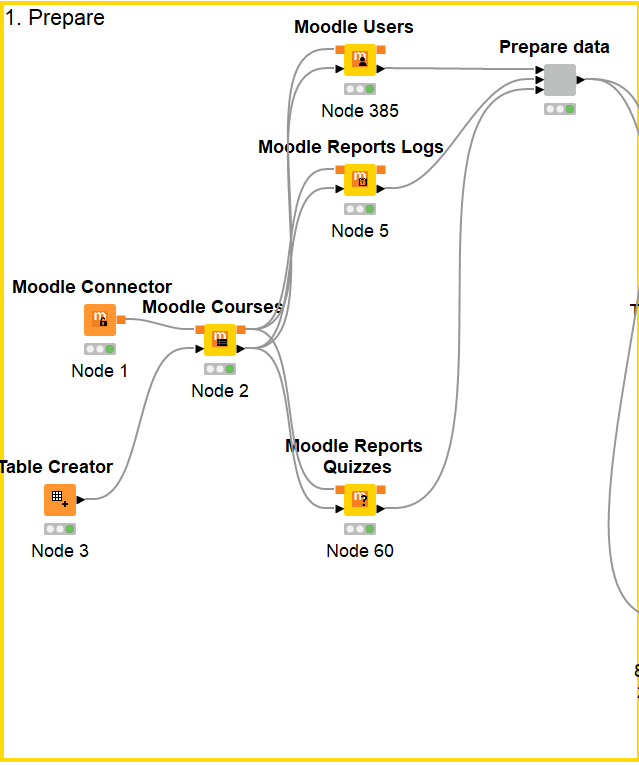
\includegraphics[width=1\textwidth]{img/workflow0.png}
	\caption{\english{Workflow}: preparación de datos.}
	\label{fig:workflow0}
\end{figure}
\FloatBarrier

Si desplegamos el componente \node{Prepare data}, veremos componentes adicionales para la extracción y tratamiento de datos específicos (Figura ~\ref{fig:workflow1}): 

\begin{figure}[!htb]
	\centering
	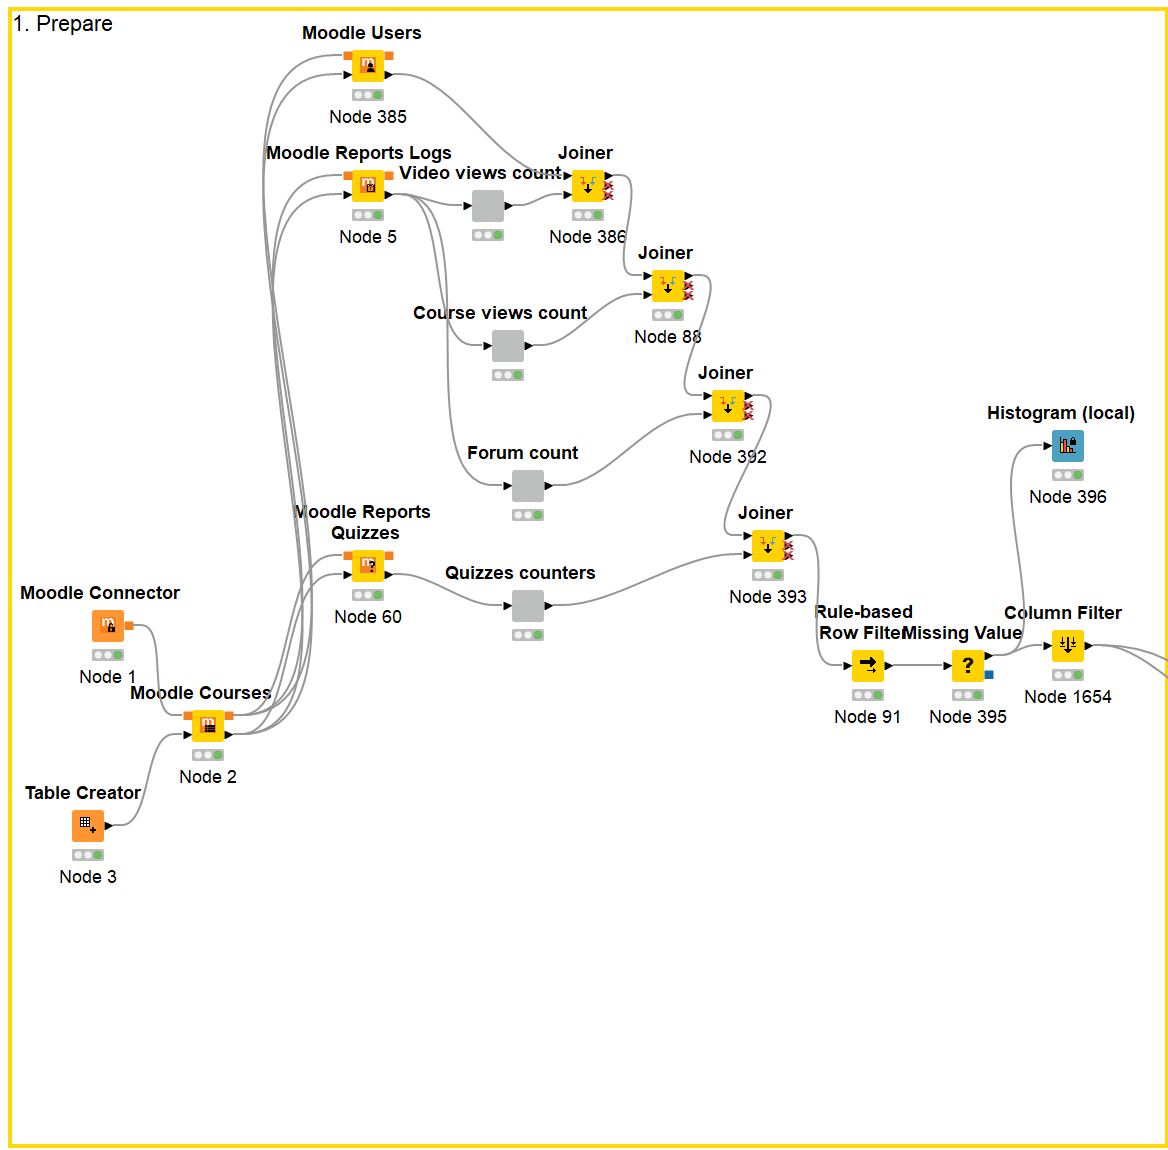
\includegraphics[width=1\textwidth]{img/workflow1.png}
	\caption{\english{Workflow}: preparación de datos (\node{Prepare data} desplegado).}
	\label{fig:workflow1}
\end{figure}
\FloatBarrier

El componente \node{Video View Count} ~\ref{fig:workflow1a} obtiene los datos de log desde el nodo \node{Moodle Reports Logs} y filtra aquellos
\english{logs} relacionados con la visualización de vídeos. Utilizando un nodo \node{GroupBy} realiza un conteo agrupando por curso y usuario, devolviendo el campo \field{videosviews}.

\begin{figure}[!htb]
	\centering
	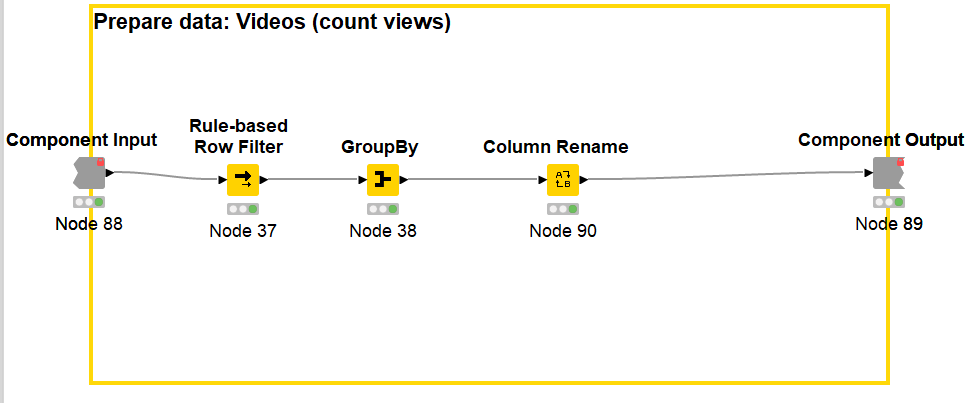
\includegraphics[width=1\textwidth]{img/workflow1a.png}
	\caption{\english{Workflow}: componente \node{Video views count}.}
	\label{fig:workflow1a}
\end{figure}
\FloatBarrier

Los componentes \node{Course views count} y \node{Forum count} funcionan de forma similar al anterior pero filtrando por los \english{logs} correspondientes a cada caso y 
devolviendo los campos \field{courseviews} y \field{forumcount} respectivamente. 

El componente \node{Quizzes counters} obtiene, a partir del nodo \node{Moodle Reports Quizzies}, información de los intentos de cuestionarios 
realizados por los usuarios y agrupa los resultados para obtener los otros campos que necesitamos \field{autoevaltotalattempts}, \field{autoevalgrademean} y la clase, \field{evalgradecategory}.

Se han realizado las siguientes operaciones de preparación y limpieza de los datos: 

\begin{itemize}
	\item Los valores nulos en calificaciones se han considerado 0. 
	\item Se han eliminado los usuarios que no han realizado ningún cuestionario de evaluación.
\end{itemize}

Tras la limpieza de datos, nos hemos quedado con un conjunto de 53 registros. En la Figura ~\ref{fig:workflow2} se muestra un fragmento de la tabla de salida con las variables necesarias para el estudio. 

\begin{figure}[!htb]
	\centering
	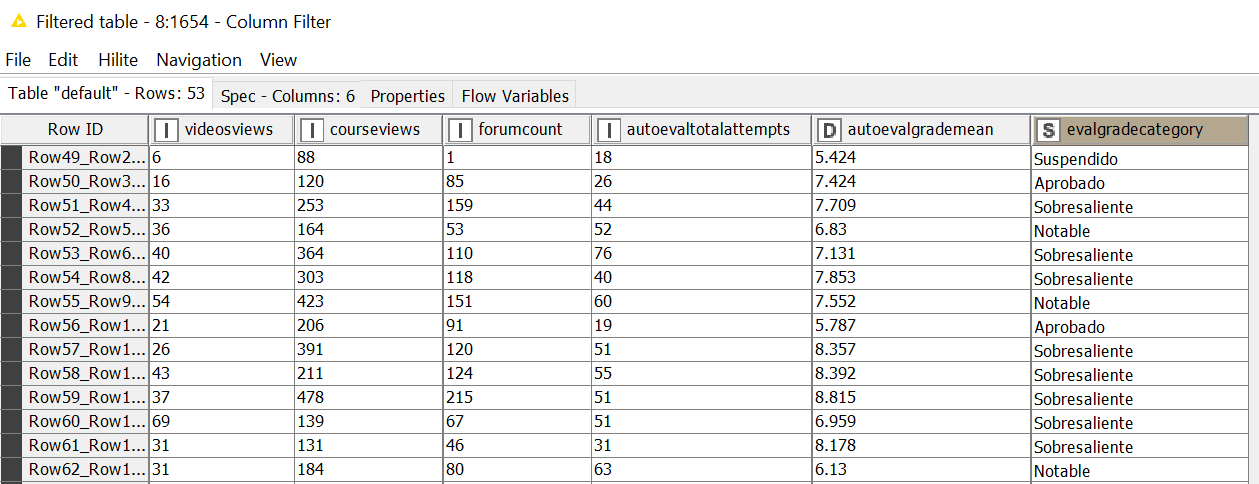
\includegraphics[width=1\textwidth]{img/workflow2.png}
	\caption{\english{Workflow}: preparación de datos (salida).}
	\label{fig:workflow2}
\end{figure}
\FloatBarrier

Como la clase es una variable cualitativa nominal, mostramos un diagrama de barras (Figura ~\ref{fig:workflow3}) con la frecuencia de cada valor posible de calificación (Suspendido, Aprobado, Notable y Sobresaliente). 

\begin{figure}[!htb]
	\centering
	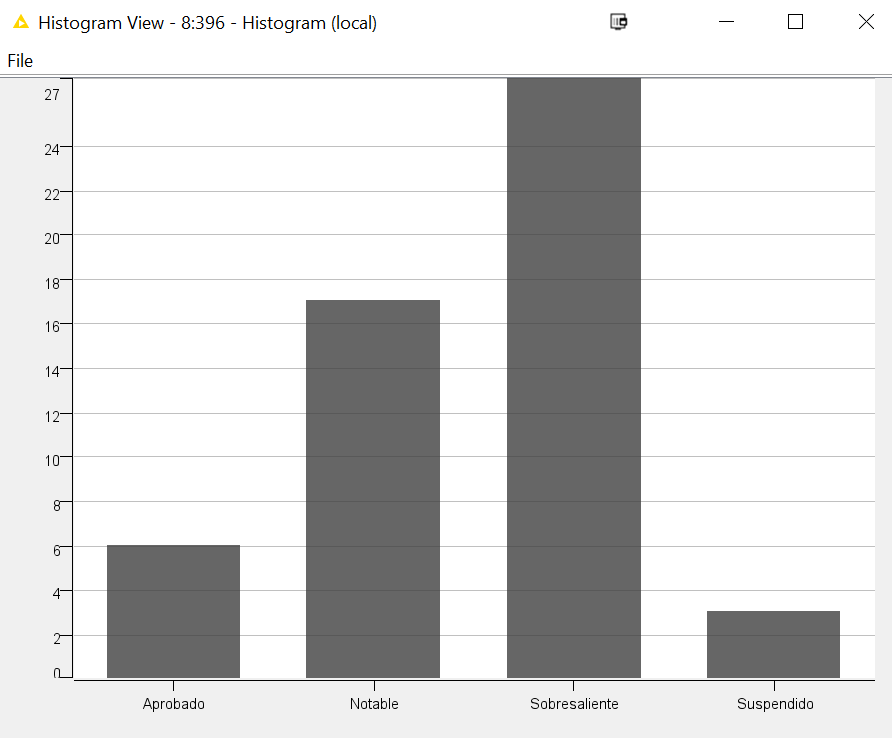
\includegraphics[width=1\textwidth]{img/workflow3.png}
	\caption{\english{Workflow}: preparación de datos (diagrama de barras clase).}
	\label{fig:workflow3}
\end{figure}
\FloatBarrier


\subsection{Modelo de aprendizaje}

En la Figura ~\ref{fig:workflow4} se muestra el \english{workflow} completo. Se han implementando tres variantes del modelo con el mismo 
objetivo, identificadas como Modelo A, Modelo B y Modelo C. 

\begin{figure}[!htb]
	\centering
	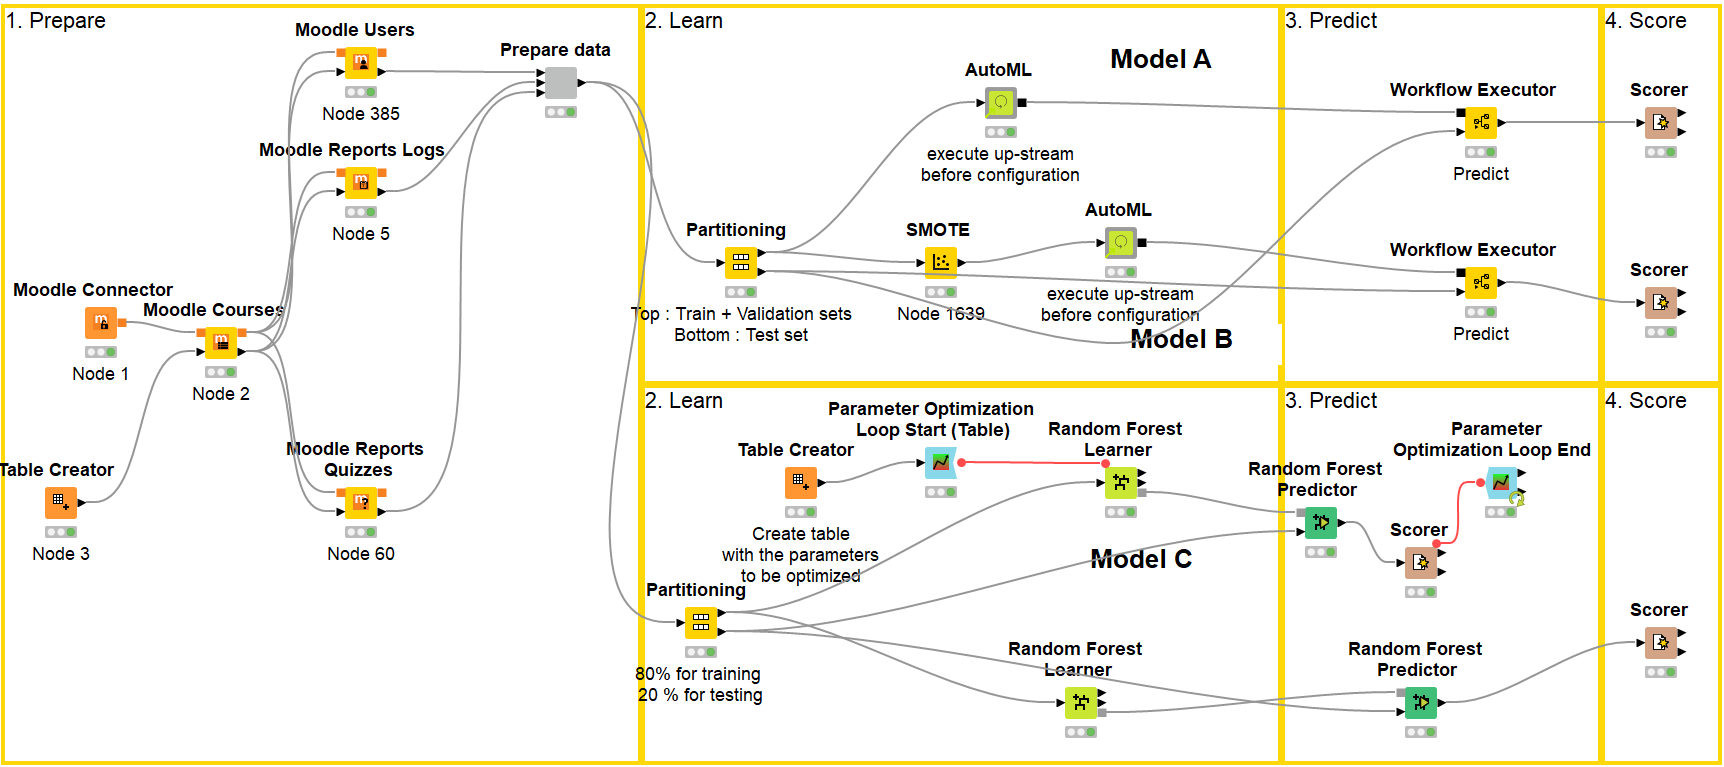
\includegraphics[width=1\textwidth]{img/workflow4.png}
	\caption{\english{Workflow} completo.}
	\label{fig:workflow4}
\end{figure}
\FloatBarrier

\subsubsection{Modelo A}

En el modelo A, mostrado en la Figura ~\ref{fig:workflowA1} utilizamos el componente \node{AutoML} de KNIME. Este componente entrena automáticamente modelos 
de aprendizaje automático supervisados para clasificación binaria o multiclase, siendo este segundo nuestro objetivo. 

El componente incluye y automatiza todo el ciclo de \english{Machine Learning}, incluyendo preparación de datos, optimización 
de parámetros con validación cruzada y evaluación y selección del mejor modelo. 

\begin{figure}[!htb]
	\centering
	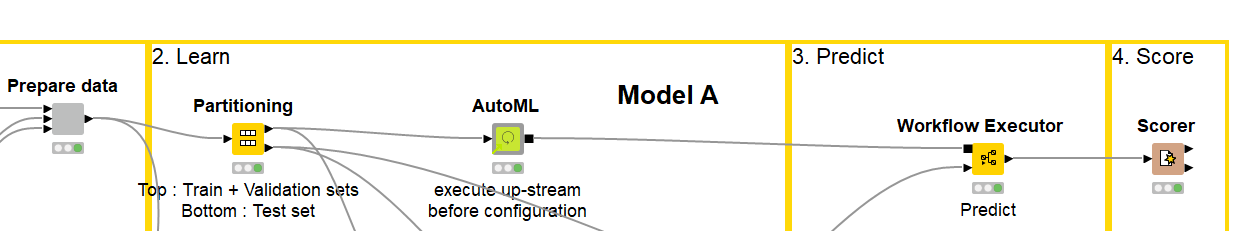
\includegraphics[width=1\textwidth]{img/workflowA1.png}
	\caption{Modelo A: \english{Workflow}.}
	\label{fig:workflowA1}
\end{figure}
\FloatBarrier

No tenemos que ver \node{AutoML} como una caja cerrada que lo hace todo por nosotros. Lo interesante está en el hecho de que 
\node{AutoML} se ha construido como un componente y no como un nodo, con lo que realmente se trata de un \english{workflow} más complejo 
que se ha agrupado como componente. Este componente puede ser expandido y podemos visualizar sus elementos y modificarlos 
según las necesidades del proyecto. 

El componente viene por defecto enlazado con el repositorio de KNIME. Esto permite, por ejemplo, actualizarlo cuando se publican nuevas versiones. 
Cuando el componente está enlazado al repositorio, podemos expandirlo y ver los elementos que lo componen, pero no podemos 
modificar su contenido. Para desenlazar el componente y, con ello, desbloquearlo, accederemos al menú contextual (clic con el botón derecho sobre el componente), y 
seleccionaremos \textbf{\english{Component} $\triangleright$ \english{Disconnect Link}}. 

En la Figura ~\ref{fig:workflowA3} se muestra el primer nivel de expansión del componente,
que a su vez está formado por otros componetes que también se pueden abrir. 

\begin{figure}[!htb]
	\centering
	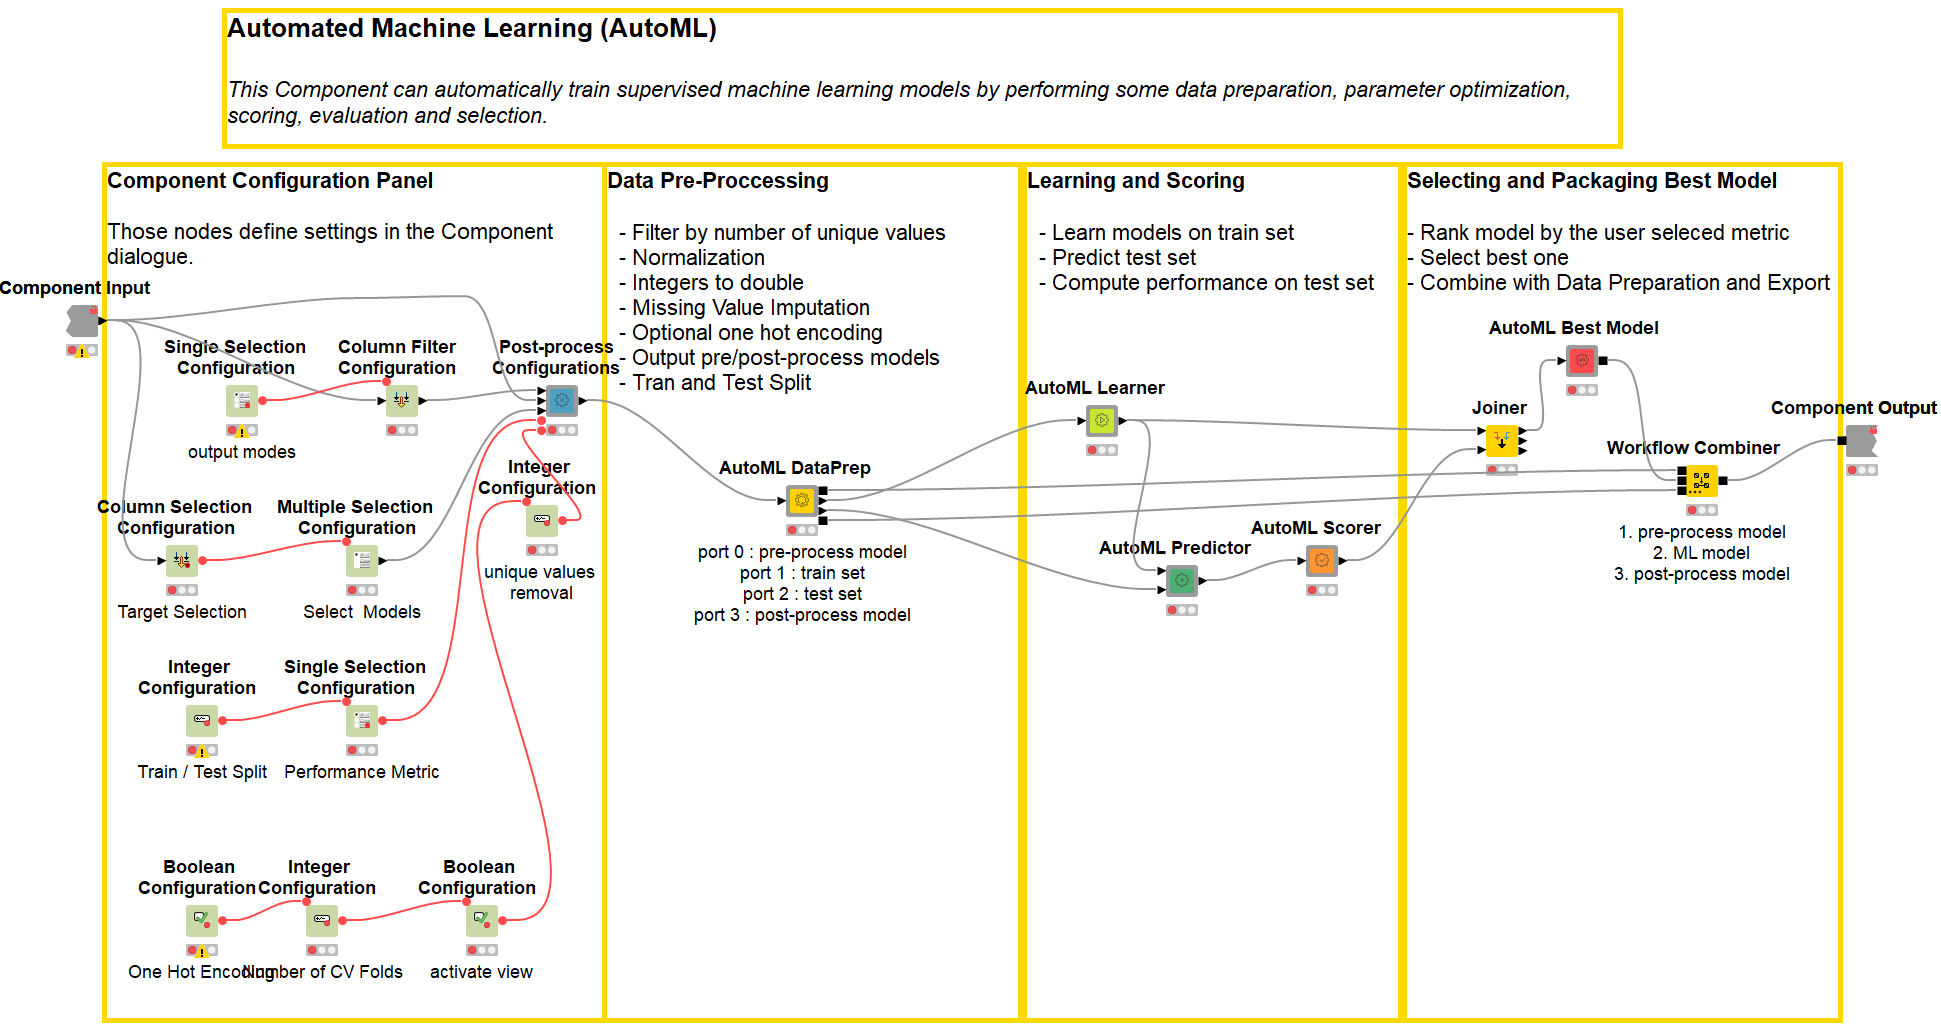
\includegraphics[width=1\textwidth]{img/workflowA3.png}
	\caption{Modelo A: Componente \node{AutoML} expandido.}
	\label{fig:workflowA3}
\end{figure}
\FloatBarrier

En la Figura ~\ref{fig:workflowA2} se muestra la configuración del componente \node{AutoML} para nuestro modelo, donde hemos seleccionado los 
modelos a entrenar: 

\begin{itemize}
	\item Naïve Bayes
	\item Logistic Regression
	\item Gradient Boosted Trees 
	\item Decision Tree 
	\item Random Forest 
	\item XGBoost Trees
\end{itemize}

\begin{figure}[!htb]
	\centering
	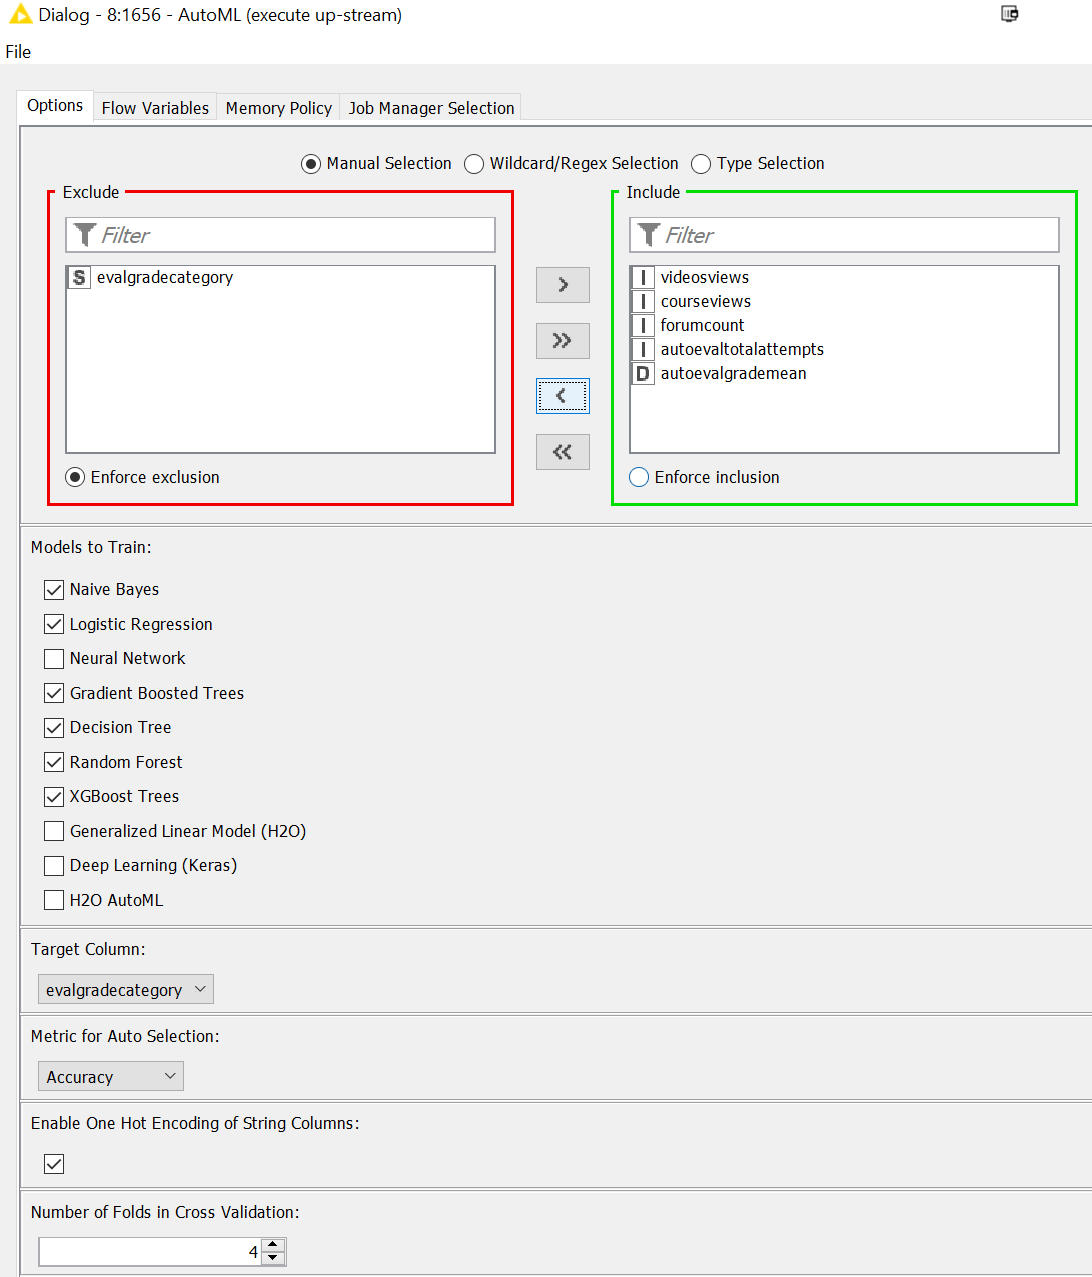
\includegraphics[width=1\textwidth]{img/workflowA2.png}
	\caption{Modelo A: Componente \node{AutoML} configuración.}
	\label{fig:workflowA2}
\end{figure}
\FloatBarrier

Como resultado de la ejecución, \node{AutoML} nos muestra un listado de los modelos ordenados por \english{Accuracy} (Figura ~\ref{fig:workflowA4}). 
Los modelos \english{Gradient Boosted Trees}, \english{Logistic Regression}, \english{Decision Tree} y \english{Random Forest} obtienen los valores más altos (\english{Accuracy} = 0.67)

\begin{figure}[!htb]
	\centering
	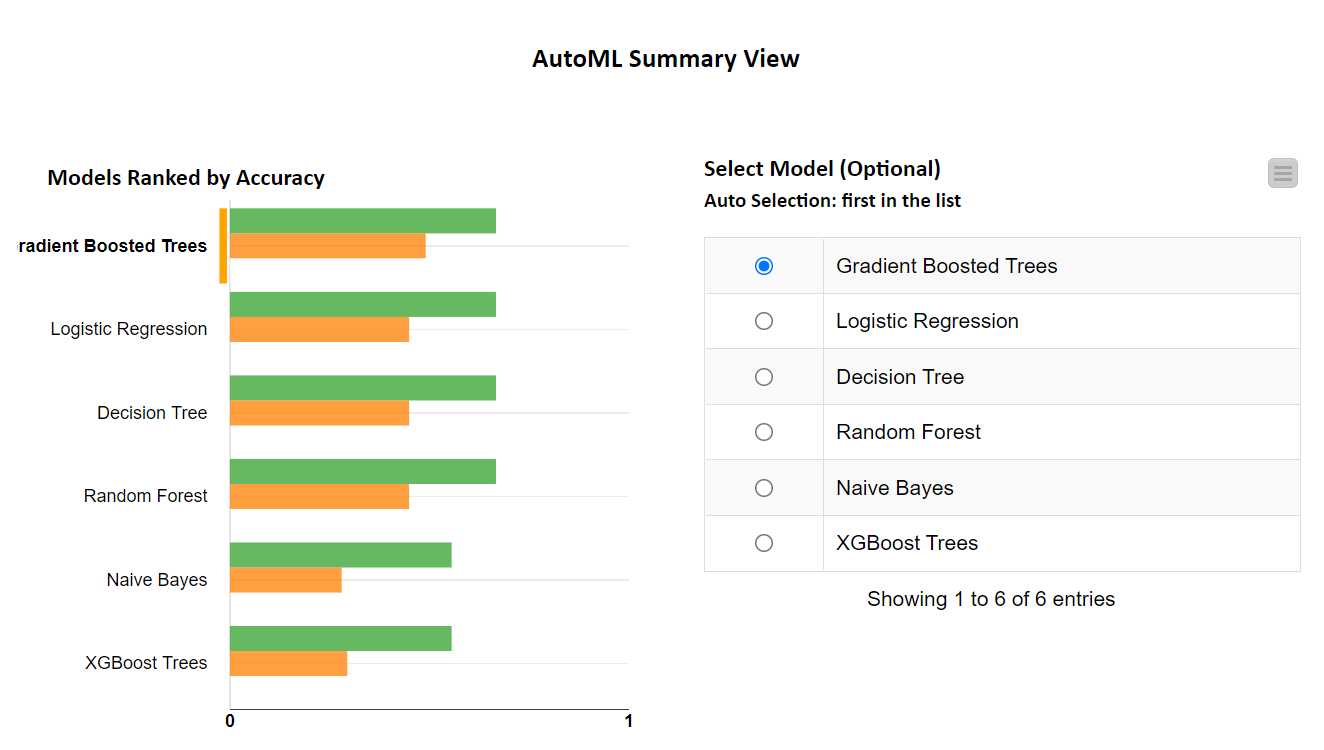
\includegraphics[width=1\textwidth]{img/workflowA4.png}
	\caption{Modelo A: Resultados (verde $\rightarrow$ \english{Accuracy}).}
	\label{fig:workflowA4}
\end{figure}
\FloatBarrier

\subsubsection{Modelo B}

El modelo B (Figura ~\ref{fig:workflowB1}) es una variante del anterior, usando también \node{AutoML}, pero añadiendo previamente sobremuestreo a los datos 
de entrada para enriquecer los datos de entrenamiento e igualar la distribución de clases. Esta técnica se llama 
\english{SMOTE} \cite{smote} (\english{Synthetic Minority Over-sampling Technique}) y KNIME dispone de un nodo que la implementa y que hemos 
configurado para que realice un sobremuestreo de las clases minoritarias. Esta técnica ha sido utilizada en otros estudios similares de 
predicción de calificaciones de estudiantes \cite{multiclass-pred}. 

\begin{figure}[!htb]
	\centering
	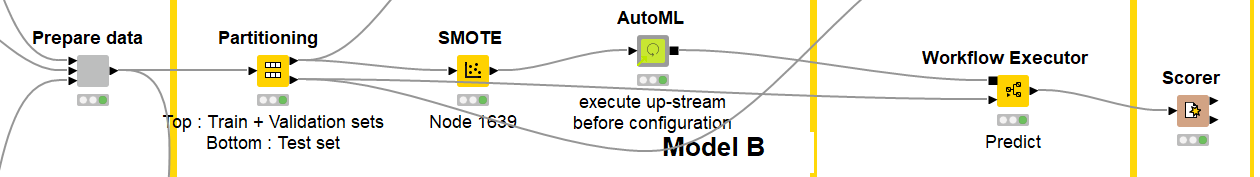
\includegraphics[width=1\textwidth]{img/workflowB1.png}
	\caption{Modelo B: \english{Workflow}.}
	\label{fig:workflowB1}
\end{figure}
\FloatBarrier

La distribución de clases ahora se muestra en la Figura ~\ref{fig:workflowB2}

\begin{figure}[!htb]
	\centering
	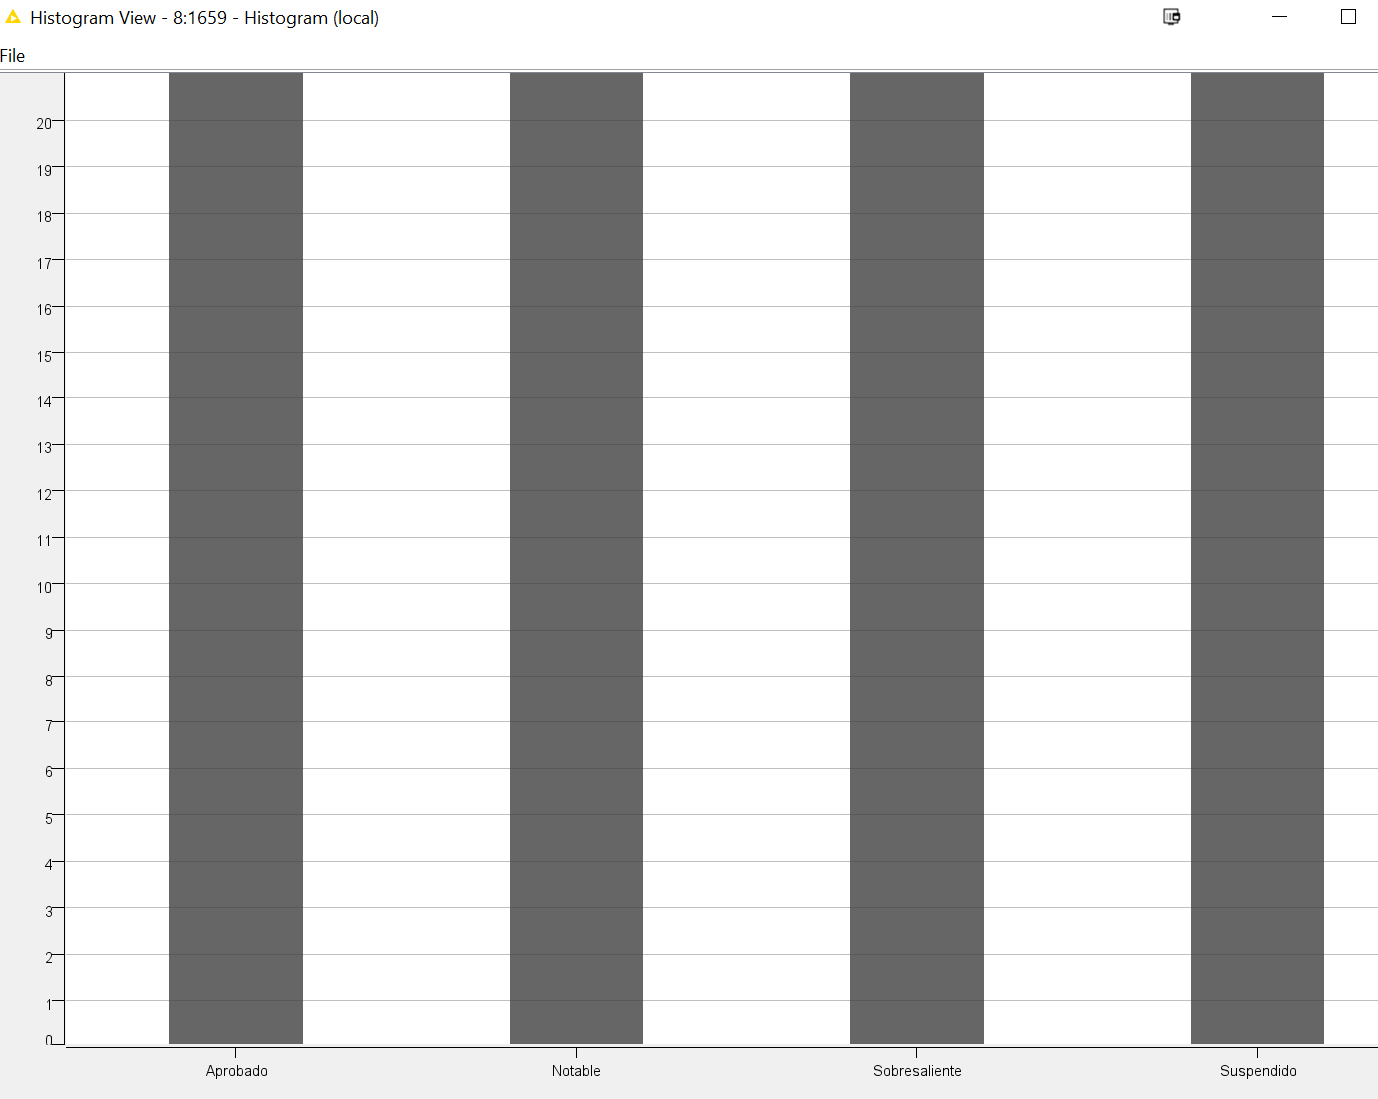
\includegraphics[width=1\textwidth]{img/workflowB2.png}
	\caption{Modelo B: \node{SMOTE}.}
	\label{fig:workflowB2}
\end{figure}
\FloatBarrier

Como resultado, vemos que se obtiene un valor mayor de \english{Accuracy} (0.76) en todos los modelos a excepción de \english{Naïve Bayes}. 

\begin{figure}[!htb]
	\centering
	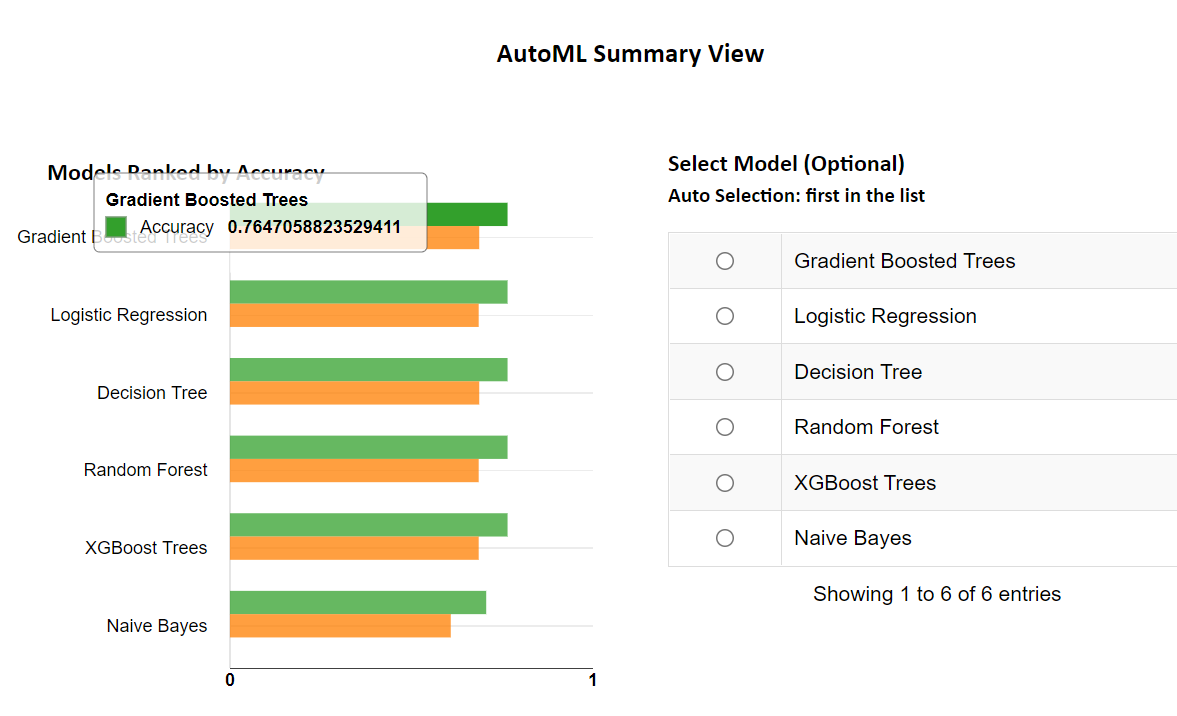
\includegraphics[width=1\textwidth]{img/workflowB3.png}
	\caption{Modelo B: Resultados (verde $\rightarrow$ \english{Accuracy}).}
	\label{fig:workflowB3}
\end{figure}
\FloatBarrier

\subsubsection{Modelo C}

En modelo C (Figura ~\ref{fig:workflowC1}) se entrena un modelo \english{Random Forest} con optimización de parámetros. 

\begin{figure}[!htb]
	\centering
	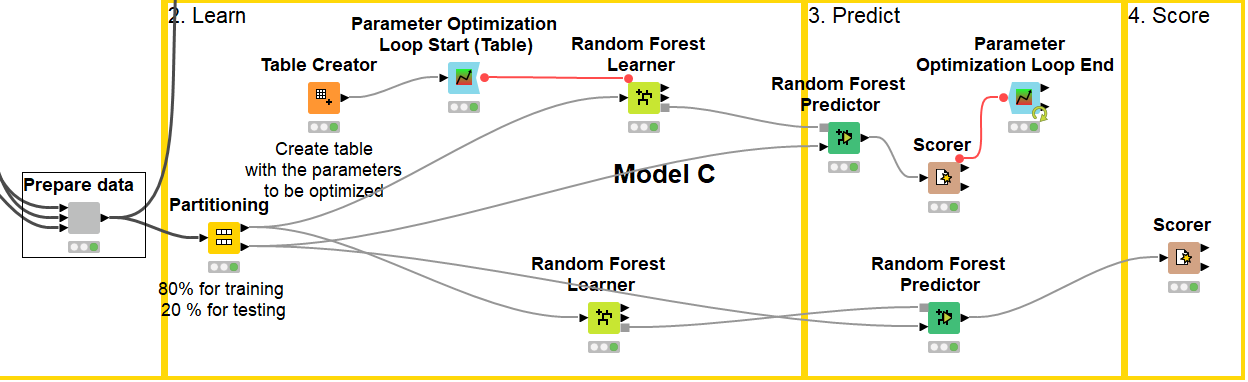
\includegraphics[width=1\textwidth]{img/workflowC1.png}
	\caption{Modelo C: \english{Workflow}.}
	\label{fig:workflowC1}
\end{figure}
\FloatBarrier

En la parte superior se observa el flujo desarrollado para ejecutar el modelo con varios parámetros y seleccionar la combinación con la 
que se obtiene un mejor valor de \english{Accuracy} (Figura ~\ref{fig:workflowC2}). 

\begin{figure}[!htb]
	\centering
	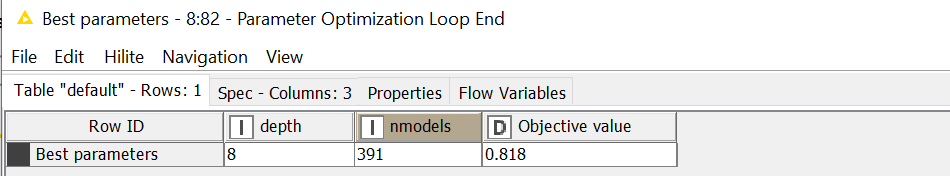
\includegraphics[width=1\textwidth]{img/workflowC2.png}
	\caption{Modelo C: \english{Best parameters}.}
	\label{fig:workflowC2}
\end{figure}
\FloatBarrier

Estos parámetros se utilizarán para configurar el modelo y obtener el modelo final. En la Figura ~\ref{fig:workflowC3} se muestra
el valor de \english{Accuracy} de este modelo (0.818) y la tabla de confusión correspondiente. 

\begin{figure}[!htb]
	\centering
	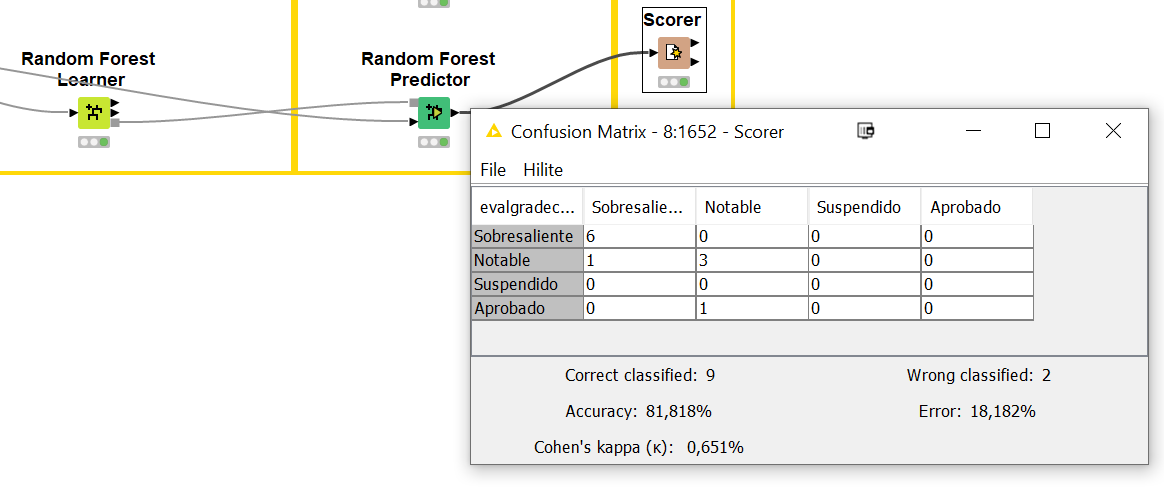
\includegraphics[width=1\textwidth]{img/workflowC3.png}
	\caption{Modelo C: Tabla de confusión.}
	\label{fig:workflowC3}
\end{figure}
\FloatBarrier


\capitulo{6}{Trabajos relacionados}

\section{UBU Monitor}

UBUMonitor es una aplicación de escritorio que permite la conexión a una plataforma Moodle para monitorizar la actividad
de los alumnos. UBUMonitor permite extraer los datos de los \english{logs} y las calificaciones obtenidas en las actividades, presentando 
los datos con herramientas de visualización que lo hacen muy atractivo. Además, añade modelos de aprendizaje automático 
para monitorizar el riesgo de abandono de los alumnos matriculados \cite{ubumonitor} \cite{marticorena2022ubumonitor}. 
\

Nuestro proyecto comparte mucho con UBUMonitor en cuando al tipo de información con la que trabaja y perfil de usuario al que
 va destinado, y nos ha resultado muy útil como referencia e incluso reutilización de algunos componentes. 
\

Sin embargo, nuestra aproximación utilizando el ecosistema de KNIME, intenta ser más abierta y flexible, dejando que sea 
el usuario final el que pueda decidir qué tipo de modelos implementar o utilizar con los datos extraídos de sus asignaturas. 



\capitulo{7}{Conclusiones y Líneas de trabajo futuras}


\section{Conclusiones}

Los objetivos generales planteados al inicio del proyecto se han podido alcanzar a la finalización del mismo, con 
lo que se ha conseguido desarrollar una extensión de KNIME muy completa que permite extraer datos de Moodle e
 incorporarlos en flujos de trabajo más complejos para estudios relacionados con la Ciencia de Datos. 
\ 

A nivel técnico se ha requerido un profundo estudio del lenguaje de programación Java, no solo orientado al desarrollo
específico de extensiones de KNIME, sino más amplio por haberse requerido integración con otras aplicaciones externas. 
También se ha ahondado en la arquitectura de KNIME, tanto a nivel de núcleo como a nivel de estructura de extensiones y nodos. 

También se han podido cumplir los objetivos personales planteados, ampliando los conocimientos adquiridos en el máster y 
aplicándolos a nuevas herramientas como KNIME y a datos de estudio de mi interés personal y de investigación, relacionados 
con la formación \english{online}. 

Sin duda, considero que se ha realizado un trabajo amplio y con mucho interés personal en la materia de estudio. 
Gracias a una tutorización continua por parte de los tutores, el proyecto ha estado muy bien organizado desde 
su inicio y se ha podido entregar una extensión de KNIME totalmente funcional, pero al mismo tiempo abierta para servir 
de base para futuras ampliaciones. 


\section{Líneas de trabajo futuras}

Debido al alcance limitado del proyecto, se han quedado fuera algunas posibles mejoras y ampliaciones, que se exponen a continuación: 

\subsection{Desarrollo de \english{plugins} de Moodle para extraer información adicional}

En este proyecto solo se ha contemplado la extracción de datos a través de las herramientas que facilita Moodle. 
Una integración más ambiciosa entre KNIME y Moodle podría conllevar el desarrollo de \english{plugins} de Moodle para extraer información más específica que no se puede extraer por defecto. 

Esta línea requiere no pensar únicamente en el rol de profesor, sino en la intervención por parte de las instituciones educativas para facilitar la integración 
y el acceso a datos adicionales. 


\subsection{Colección de Flujos de trabajo de KNIME para Moodle}

KNIME permite crear flujos de trabajo y compartirlos, de forma que sea fácil su reutilización. Se propone en esta línea crear un set de 
\english{workflows} ya preparados para su utilización con la extensión de Moodle desarrollada. 


\subsection{KNIME en servidor}

Los flujos de trabajo estudiados en este proyecto se basan en la ejecución local de una instancia de KNIME. La propuesta es utilizar 
KNIME en \english{cloud} o servidor para flujos de trabajo que actúan de forma permanente. Por ejemplo, un flujo que revisa constantemente la evolución de un curso para 
determinar si algún alumno está en riesgo de abandono. 

\subsection{Comunicación bidireccional entre KNIME y Moodle}

En este proyecto solo se ha contemplado la extracción de datos desde Moodle hacia KNIME. Moodle permite, a través de determinados 
servicios web ya incluidos o a través de servicios web personalizados, realizar acciones en el aula. Sería interesante que el resultado 
de la ejecución de un \english{workflow} de KNIME pudiera realizar acciones a partir de los resultados obtenidos. Por ejemplo, enviar un correo a
 los alumnos clasificados como en riesgo de abandono o publicar un mensaje de aviso en el foro del aula. 
 
\subsection{Datos Abiertos (Open Data)}

Conseguir que las instituciones educativas involucradas en el proyecto faciliten datos abiertos de forma automática con una política previa de anonimización (Open Data). 
Aunque existen intentos de publicar información basados en la información estrictamente legal (portal de transparencia) y datos preprocesados 
con estadísticas finales, con el auge de la Ciencia de Datos, se hace cada vez más necesario el acceso a datos en bruto para análisis más variados. 

\subsection{Anonimización}

Realizar una anonimización ajustada a la política de anonimización de la institución y que cubra la anonimización de identificadores de usuarios. 


\subsection{Obtener género}

Mejorar la API incluyendo varios proveedores externos. 


\subsection{Desvincular de librerías externas}

Eliminar las dependencias con las librerías externas. Por ejemplo, eliminar el código dependiente de UBUMonitor desarrollando soluciones propias integradas en la extensión. 

\subsection{Actualización}

Actualización a la última versión de KNIME, actualmente la 5.x. Definir un plan de mantenimiento y actualizaciones a versiones futuras. Se debe comprobar 
si alguna de las librerías y componentes utilizados en nuestro proyecto han quedado obsoletas y requieren ser sustituidas. 


\subsection{Ampliación de funcionalidad}

Ampliar funcionalidad extrayendo más información disponible en Moodle. Por ejemplo, la versión actual está limitada en los tipos de logs que se extraen. 


\subsection{Ampliar pruebas}

Las pruebas que se han llevado a cabo han estado muy dirigidas hacia un tipo de cursos y una plataforma Moodle concreta. Se considera necesario 
ampliar las pruebas a otros entornos de Moodle y otros tipos de acciones formativas. 


\subsection{Compartir extensión}

Compartir la extensión en el \english{Community} HUB para que esté disponible para otros usuarios de la comunidad. 





\counterwithin{figure}{section}

%\renewcommand\chaptername{Anexo}
%\renewcommand\thechapter{\Roman{chapter}}
%\setcounter{chapter}{0}

% Añadir entrada en el índice: Anexos
\appendix
\addcontentsline{toc}{part}{Apéndices}
\part*{Apéndices}

\apendice{Plan de Proyecto Software}
\label{sec:appendixA}

\section{Metodología}

Durante el desarrollo de este proyecto se ha utilizado una versión simplificada de la metodología Scrum. Concretamente se han
seguido ciclos o \english{sprints} de dos semanas, apoyados por reuniones de coordinación con los tutores del proyecto. Tras cada \english{sprint} se 
han mostrado y discutido los avances realizados y se han planificado las tareas a realizar en el siguiente \english{sprint}. 
\

Aunque durante el desarrollo del proyecto se han producido retrasos que han llevado a dilatar la 
entrega final del proyecto, el orden de ejecución de los \english{sprints} y el alcance del proyecto se han 
mantenido según la planificación inicial, que se detalla a continuación. 


\section{Planificación temporal}

En este apartado se describen las tareas llevadas a cabo en cada \english{sprint}. 

\subsection{\english{Sprint} 0}

\english{Sprint} de arranque del proyecto dedicado al análisis del problema y el alcance de la solución. 

\begin{itemize}
	\item Preparación del entorno de desarrollo para programar extensiones de KNIME.
	\item Desarrollo de nodo de prueba para conocer la arquitectura de KNIME.
\end{itemize}

Fechas: desde 02/02/2022 a 15/02/2022.

\subsection{\english{Sprint} 1}

En este \english{sprint} continuamos con la fase de análisis: 

\begin{itemize}
	\item Preparación de plataforma Moodle local con datos de prueba. 
	\item Pruebas de acceso a la información de Moodle a través de \english{web services} y \english{web scraping}. 
    \item Estudio de la aplicación UBUMonitor, tanto a nivel de usuario como a nivel de código, para evaluar su posible reutilización.
    \item Se define el alcance y objetivos del proyecto.
    \item Memoria: se prepara el documento base de memoria y se completan los apartados de Introducción, Objetivos y Análisis. 
\end{itemize}

Fechas: desde 27/04/2022 a 10/05/2022.

\subsection{\english{Sprint} 2}

\english{Sprint} dedicado al diseño de algunos de los módulos propuestos durante la fase de análisis. 

\begin{itemize}
	\item Diseño de nodo \node{Moodle Connection}.
	\item Diseño de nodo \node{Moodle Courses}.
	\item Diseño de nodo \node{Moodle Users}.
	\item Memoria: documentación parcial de los apartados de Técnicas y herramientas y Diseño.
\end{itemize}

Fechas: desde 11/05/2022 a 24/05/2022.

\subsection{\english{Sprint} 3}

Implementación parcial de los nodos diseñados en el \english{sprint} anterior. En este \english{sprint} los nodos implementados son operativos 
pero no se ha añadido aún configuración. 

\begin{itemize}
	\item Implementación parcial del nodo \node{Moodle Connection}.
	\item Implementación parcial del nodo \node{Moodle Courses}.
	\item Implementación parcial del nodo \node{Moodle Users}.
	\item \english{Workflow} básicos para probar los nodos implementados con datos de prueba de Moodle. 
	\item Memoria: documentación parcial del apartado de Implementación.
\end{itemize}

Fechas: desde 25/05/2022 a 07/06/2022.

\subsection{\english{Sprint} 4}

Ampliación de los nodos implementados en el \english{sprint} anterior añadiendo configuración. 

\begin{itemize}
	\item Implementación de configuración del nodo \node{Moodle Connection}.
	\item Implementación de configuración del nodo \node{Moodle Courses}.
	\item Implementación de configuración del nodo \node{Moodle Users}.
	\item Memoria: actualización del apartado de Implementación. 
\end{itemize}

Fechas: desde 08/06/2022 a 21/06/2022.

\subsection{\english{Sprint} 5}

\english{Sprint} dedicado al diseño de otros módulos propuestos durante la fase de análisis. 

\begin{itemize}
	\item Diseño del nodo Moodle Reports Logs y primeras pruebas de implementación. 
	\item Memoria: actualización del apartado de Diseño.
\end{itemize}

Fechas: desde 22/06/2022 a 05/07/2022.

\subsection{\english{Sprint} 6}

\english{Sprint} dedicado a la implementación del nodo \node{Moodle Reports Logs}. 

\begin{itemize}
	\item Implementación del nodo \node{Moodle Reports Logs}. 
	\item Mapeo de \english{logs} de Moodle para extraer variables de los textos de \english{log}. 
	\item Memoria: actualización del apartado de Implementación. 
\end{itemize}

Fechas: desde 06/07/2022 a 07/08/2022.

\subsection{\english{Sprint} 7}

\english{Sprint} dedicado al diseño de otros módulos propuestos durante la fase de análisis. 

\begin{itemize}
	\item Diseño del nodo \node{Moodle Reports Grades} y primeras pruebas de implementación. 
	\item Memoria: actualización del apartado de Diseño.
\end{itemize}

Fechas: desde 25/01/2023 a 06/02/2023.

\subsection{\english{Sprint} 8}

\english{Sprint} dedicado a la implementación del nodo \node{Moodle Reports Grades}. 

\begin{itemize}
	\item Implementación del nodo \node{Moodle Reports Grades}. 
	\item Memoria: actualización del apartado de Implementación. 
\end{itemize}

Fechas: desde 23/08/2023 a 05/09/2023.

\subsection{\english{Sprint} 9}

\english{Sprint} dedicado a la ampliación del nodo \node{Moodle Users}. 

\begin{itemize}
	\item Incorporación de anonimización de usuarios.
	\item Estimación de género de usuario. 
	\item Memoria: actualización del apartado de Implementación. 
\end{itemize}

Fechas: desde 06/09/2023 a 19/09/2023.

\subsection{\english{Sprint} 10}

\english{Sprint} dedicado a la preparación final del código y compilación de la solución final. 

\begin{itemize}
	\item Limpieza del código eliminando mensajes de depuración y añadiendo comentarios.
	\item Compilación final para generar el plugin que puede ser utilizado en cualquier \english{workflow} de KNIME. 
	\item Memoria: actualización del apartado de Implementación. 
\end{itemize}

Fechas: desde 20/09/2023 a 03/10/2023.

\subsection{\english{Sprint} 11}

Primer \english{sprint} dedicado al uso de los nodos implementados con datos reales. 

\begin{itemize}
	\item Importación de datos reales en Moodle local. 
	\item Implementación de \english{workflows} básicos para probar el correcto acceso a datos reales. 
	\item Memoria: actualización del apartado de \english{Workflows}. 
\end{itemize}

Fechas: desde 04/10/2023 a 17/10/2023.


\subsection{\english{Sprint} 12}

\english{Sprint} dedicado a la implementación del \english{Workflow} con datos reales. 

\begin{itemize}
	\item Implementación del \english{worflow} con datos reales. 
	\item Memoria: actualización del apartado de \english{Workflows}. 
\end{itemize}

Fechas: desde 18/10/2023 a 31/10/2023.

\subsection{\english{Sprint} 13}

\english{Sprint} dedicado a la implementación del \english{Workflow} con datos reales (continuación). 

\begin{itemize}
	\item Implementación del \english{worflow} con datos reales. 
	\item Memoria: actualización del apartado de \english{Workflows}. 
	\item Memoria: revisión general. 
\end{itemize}

Fechas: desde 02/11/2023 a 14/11/2023.

\subsection{\english{Sprint} 14}

\english{Sprint} dedicado a completar la memoria del proyecto. 

\begin{itemize}
	\item Memoria: actualización de apartados pendientes
	\item Memoria: corrección general según sugerencias reportadas en el \english{sprint} anterior. 
\end{itemize}

Fechas: desde 15/11/2023 a 28/11/2023.

\newpage
\section{Estudio de viabilidad}

\subsection{Viabilidad económica}
\subsubsection{Costes de personal}
Aunque el proyecto se ha estimado en 7 meses a tiempo parcial, para calcular el coste del proyecto, se 
considerará que se ha realizado por un desarrollador a tiempo completo en un período de 3,5 meses. 
Se considera el salario medio neto de un programador de 1.610 € mensuales \cite{salario}.
(ver tabla~\ref{tab:personal}).

La cotización a la seguridad social se ha calculado como horas comunes, según
el régimen general de 2023 (28,30\%)~\cite{seguridad-social}.

\begin{table}[!h]
	\centering
	\begin{tabular}{lr}
		\toprule
		\textbf{Concepto} & \textbf{Coste} \\
		\midrule
		Salario neto & 1.610,00 €\\
		Retención IRPF (17\%) & 500,37 € \\
		Seguridad social (28,30 \%) & 832,96 € \\
		\midrule
		Salario bruto (mensual) & 2.943,33 € \\
		\midrule
		\textbf{Total 3.5 meses} & 10.301,65 \\
		\bottomrule
	\end{tabular}
	\caption{Costes de personal.}
	\label{tab:personal}
\end{table}

Además se sumará el sueldo de los dos tutores asignados al proyecto \cite{misc:retribuciontutores-funcionarios} durante 7 meses, ambos con la posición de Profesor Titular de Universidad. Se asignan 0,5 por tutor.

Sueldo mensual: 3.145,59 €. Imparte 24 créditos anuales.
$$ \dfrac{\textup{3.145,59 €} \times 12 \;meses}{24 
	\;créditos} \times 0,5 \;créditos \times 2 \;tutores = \textup{1.572,80 €} $$


El coste de los tutores corresponde a 1.572,80 €.

\subsubsection{Costes de \textit{hardware}}
En esta sección se enumeran los costes del \textit{hardware} usado durante el desarrollo.

Para el desarrollo se ha usado un equipo de sobremesa valorado en 1.200 €, con 
amortización en 4 años (ver tabla~\ref{tab:hardware}).

$$\dfrac{\textup{1200 €}}{4 \;años * 12 \;meses} = 
\textup{25} $$

\begin{table}[!h]
	\centering
	\begin{tabular}{lrr}
		\toprule
		\textbf{Concepto} & \textbf{Coste} & \textbf{Amortización} \\
		\midrule
		Ordenador sobremesa & 1.200 € & 25 \\
		\midrule
		\textbf{Total 3,5 meses} & 87,5 € \\
		\bottomrule
	\end{tabular}
	\caption{Costes de hardware.}
	\label{tab:hardware}
\end{table}

\subsubsection{Costes totales}

En la tabla~\ref{tab:total} se agrupan todos los costes calculados del proyecto, dando el total de  €.

\begin{table}[!h]
	\centering
	\begin{tabular}{lr}
		\toprule
		\textbf{Concepto} & \textbf{Coste} \\
		\midrule
		Personal & 10.301,65 € \\
		Tutores  & 1.572,80 € \\
		\textit{Hardware} & 87,51 € \\
		\midrule
		\textbf{Total} & 11.961,96 € \\
		\bottomrule
	\end{tabular}
	\caption{Costes totales del proyecto.}
	\label{tab:total}
\end{table}

\subsection{Viabilidad legal}

KNIME es una herramienta de software libre que puede ser descargada y utilizada gratuitamente bajo los 
términos de la Licencia Pública General de GNU versión 3 (GPLv3). Hay que tener en cuenta que, aunque la 
plataforma es gratuita, algunas extensiones de terceros pueden tener licencias específicas y 
restricciones de uso. En este proyecto se han utilizado extensiones adicionales de KNIME para 
definir los \english{workflows} de trabajo, pero no se han requerido estas extensiones dentro del código 
de la extensión y nodos desarrollados, por lo que solo se deben tener en cuenta los términos de la
 licencia GPLv3 del núcleo de KNIME. 

Adicionalmente se ha incluido código de la aplicación externa UBUMonitor, distribuido bajo licencia MIT. Esta licencia permite, entre 
otras cosas, la modificación, distribución y uso comercial del código fuente, por lo que el código 
de UBUMonitor se puede incorporar a nuestro proyecto sin restricciones, pero a su vez sin garantías de ningún tipo. 


\apendice{Especificación de requisitos}
\label{sec:appendixB}

\section{Introducción}

En este apéndice se detallan sus requisitos, tanto funcionales como no funcionales.

\section{Catálogo de requisitos}
\subsection{Requisitos funcionales}

\begin{itemize}
	\item \textbf{RF-1 Conexión}: la extensión debe poder conectarse con cualquier plataforma Moodle.
    \begin{itemize}
		\item \textbf{RF-1.1 Conexión: Rol profesor}: el usuario debe tener el rol profesor en la plataforma.
		\item \textbf{RF-1.2 Conexión: APP móvil}:  la plataforma Moodle debe tener el acceso a la aplicación móvil activado.
	\end{itemize}

	\item \textbf{RF-2 Consulta de cursos}: la debe ser capaz de extraer información de los cursos de la plataforma Moodle.
    \begin{itemize}
		\item \textbf{RF-2.1 Filtro por identificador de curso}: la extensión debe poder extraer un curso específico, indicando su \field{id} dentro de la plataforma Moodle.
		\item \textbf{RF-2.2 Filtro por identificador de categoría}: la extensión debe poder extraer todos los cursos de una categoría, indicando su \field{id} dentro de la plataforma Moodle.
	\end{itemize}

	\item \textbf{RF-3 Consulta de usuarios}: la extensión debe de extraer información de los usuarios de la plataforma Moodle.
	\item 	\begin{itemize}
		\item \textbf{RF-3.1 Filtro de usuarios por curso}: la extensión debe poder extraer los usuarios de un curso específico o de un listado de cursos. 
		\item \textbf{RF-3.2 Filtro de usuarios por rol}: la extensión debe poder filtrar solo por usuarios con el rol Estudiante. 
		\item \textbf{RF-3.3 Estimación del género del estudiante}: la extensión debe poder estimar el género del estudiante a partir de su nombre. 
		\item \textbf{RF-3.4 Anonimización de datos personales}: la extensión debe poder anonimizar los datos personales del usuario (nombre y apellidos). 
	\end{itemize}
	\item \textbf{RF-4 Consulta de logs}: la extensión debe ser capaz de extraer los logs de los cursos indicados. 
	\item \textbf{RF-5 Consulta de calificaciones}: la extensión debe ser capaz de extraer las calificaciones de los usuarios registrados en los cursos indicados. 
	\item \textbf{RF-6 Consulta de cuestionarios}: la extensión debe ser capaz de extraer información de los cuestionarios de los usuarios registrados en los cursos indicados. 
\end{itemize}

\subsection{Requisitos no funcionales}
\begin{itemize}
	\item \textbf{RNF-1 Usabilidad}: los nodos desarrollados deben ser intuitivos y fáciles de usar, siguiendo el diseño de otros nodos y extensiones de KNIME.
	\item \textbf{RNF-2 Mantenibilidad}: debe ser sencillo añadir funcionalidad adicional, siguiendo las recomendaciones de desarrollo de extensiones de KNIME.
	\item \textbf{RNF-3 Compatibilidad}: la extensión desarrollada debe ser compatible con la versión de KNIME 4.7.
\end{itemize}
\apendice{Especificación de diseño}
\label{sec:appendixC}

\section{Introducción}

En este apéndice se describen los diseños de nodos que permiten cumplir con los objetivos
 generales del proyecto y los requisitos funcionales definidos previamente. 

\section{Diseño de la extensión KNIME Moodle Integration}

Se ha diseñado la extensión KNIME Moodle Integration con los siguientes nodos individuales: 

\begin{itemize}
  \item \node{Moodle Connector}. Cubre los requisitos especificados en RF-1 (RF-1.1 y RF-1.2). 
  \item \node{Moodle Courses}. Cubre los requisitos especificados en RF-2 (RF-2.1 y RF-2.2).
  \item \node{Moodle Users}. Cubre los requisitos especificados en RF-3 (RF-3.1, RF-3.2, RF-3.3 y RF-3.4).
  \item \node{Moodle Reports Logs}. Cubre los requisitos especificados en RF-4. 
  \item \node{Moodle Reports Grades}. Cubre los requisitos especificados en RF-5. 
  \item \node{Moodle Reports Quizzes}. Cubre los requisitos especificados en RF-6. 
\end{itemize}

En el diseño se han tenido en cuenta también los requisitos no funcionales RNF-1, RNF-2 y RNF-3. 
\

\begin{figure}[!h]
	\centering
	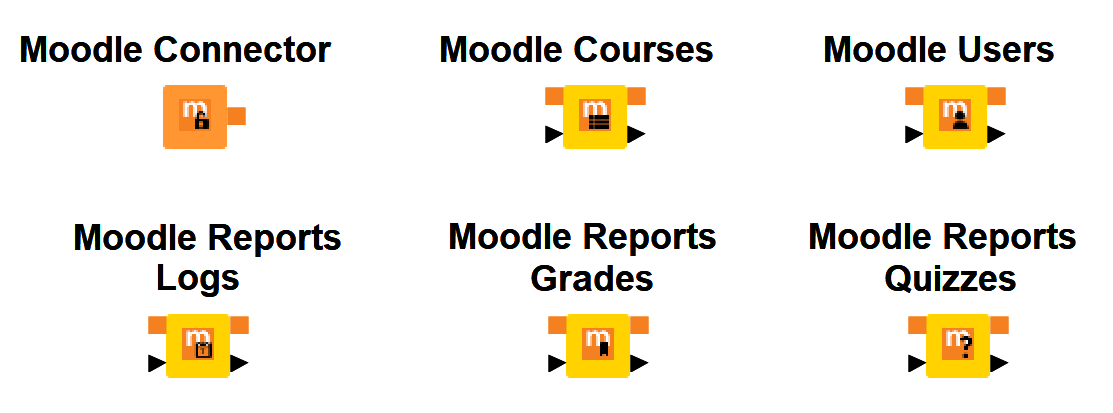
\includegraphics[width=1\textwidth]{img/nodes_moodle_todos.png}
	\caption{Nodos implementados en la extensión \node{KNIME Moodle Integration}.}
	\label{fig:moodlenodesall}
\end{figure}
\FloatBarrier


Se describe a continuación el diseño de cada nodo implementado. 

\newpage
\subsection{Diseño del nodo Moodle Connector}

El nodo \node{Moodle Connector} establece la conexión con una plataforma Moodle. Requiere una cuenta con perfil de profesor (RF-1.1). 
Requiere que la plataforma Moodle tenga activado el acceso a la aplicación móvil (RF-1.1). 
\

El nodo devuelve a través de un puerto de salida la información de sesión, de forma que, conectada a otros nodos de la extensión, 
estos pueden extraer información de Moodle sin necesidad de volver a conectarse.
\ 

El nodo tiene la siguiente \textbf{estructura}:

\begin{itemize}
	\item \textbf{Puertos de entrada}: 
    \begin{itemize}
		\item Sin puertos de entrada. 
   	\end{itemize}

	\item \textbf{Puertos de salida}: 
    \begin{itemize}
		\item \textbf{0. Moodle Courses}. Una conexión que se puede utilizar para acceder a la API de Moodle. 
   	\end{itemize}

\end{itemize}

\begin{figure}[!h]
	\centering
	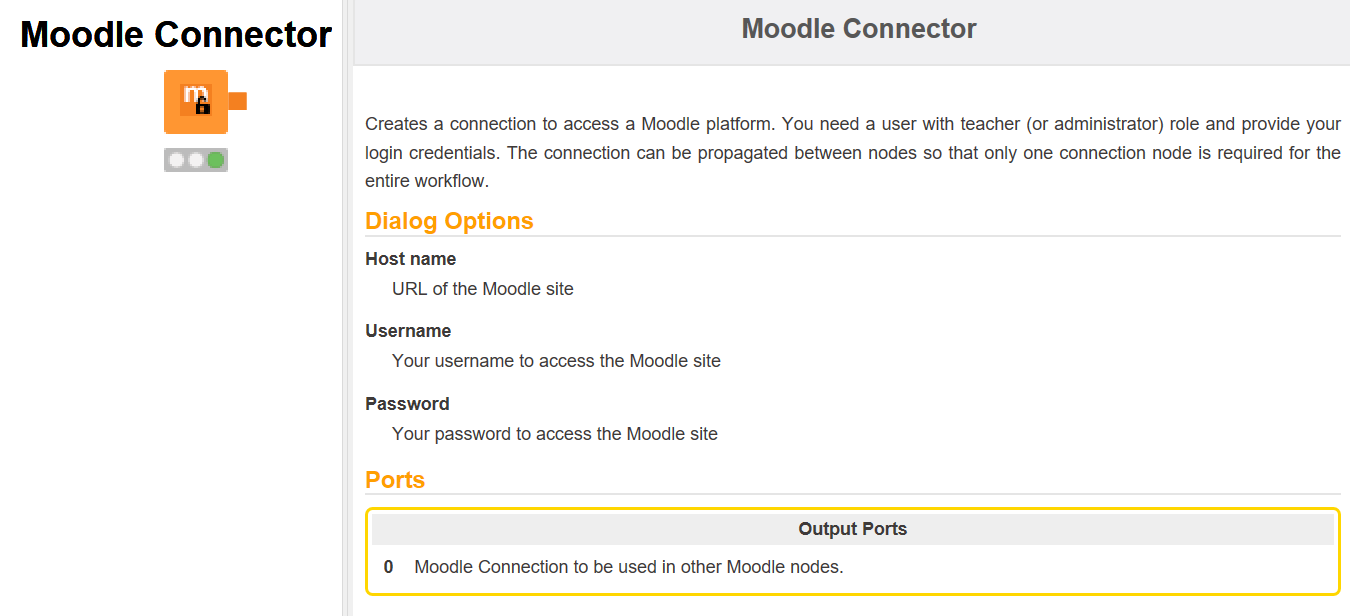
\includegraphics[width=1\textwidth]{img/nodes_moodle_connector.png}
	\caption{Nodo \node{Moodle Connector}. Descripción.}
	\label{fig:moodleconnector}
\end{figure}
\FloatBarrier


El nodo permite la siguiente \textbf{configuración}: 

\begin{itemize}
   \item \textbf{Host name}. URL de la plataforma Moodle, empezando por http o https. 
   \item \textbf{Username}. Nombre de usuario de acceso a Moodle.
   \item \textbf{Password}. Contraseña de acceso a Moodle.
\end{itemize}

\begin{figure}[!h]
	\centering
	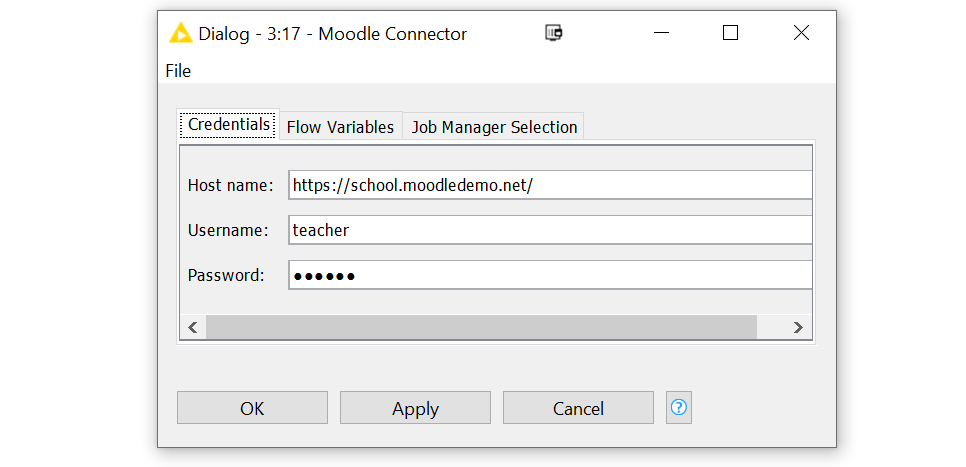
\includegraphics[width=1\textwidth]{img/nodes_moodle_connector_settings.png}
	\caption{Nodo \node{Moodle Connector}. Configuración.}
	\label{fig:moodleconnector_settings}
\end{figure}
\FloatBarrier

\hphantom{ }

\newpage    
\subsection{Diseño del nodo Moodle Courses}

El nodo \node{Moodle Courses} extrae información de cursos. Permite obtener uno o varios cursos según su id (RF-2.1) o todos 
los cursos dentro de las categorías especificadas (RF-2.2). 
\

El nodo tiene la siguiente \textbf{estructura}:

\begin{itemize}
	\item \textbf{Puertos de entrada}: 
    \begin{itemize}
		\item \textbf{0. Moodle Connection}. Conexión obtenida desde el nodo \node{Moodle Connector}. 
		\item \textbf{1. Input table}. Tabla de entrada con información de filtrado. 
		Columna con identificador de cursos y columna con identificador de categorías. Aunque el filtrado no es obligatorio, sí se 
		requiere añadir un nodo que defina la tabla de entrada. 
   	\end{itemize}

	\item \textbf{Puertos de salida}: 
    \begin{itemize}
		\item \textbf{0. Moodle Connection}. Devuelve la conexión para facilitar su transferencia al siguiente nodo del flujo de trabajo. 
		\item \textbf{1. Output table}. Tabla de salida con la información de los cursos. 
   	\end{itemize}

\end{itemize}

\begin{figure}[!h]
	\centering
	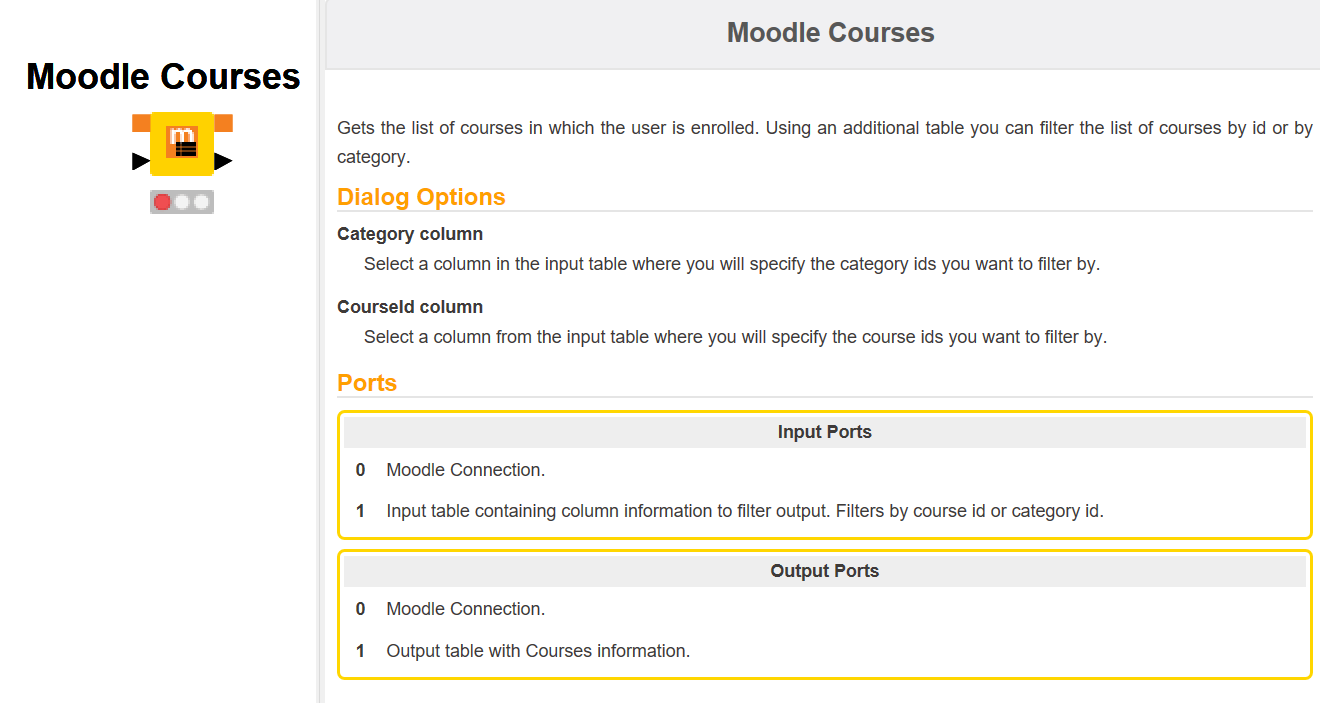
\includegraphics[width=1\textwidth]{img/nodes_moodle_courses.png}
	\caption{Nodo \node{Moodle Courses}. Descripción.}
	\label{fig:moodlecourses}
\end{figure}
\FloatBarrier



El nodo permite la siguiente \textbf{configuración}: 

\begin{itemize}
   \item \textbf{Category column}. Permite seleccionar la columna en la que se encuentran las categorías por las que se desea filtrar. Es opcional. 
   \item \textbf{CourseId column}. Permite seleccionar la columna en la que se encuentran los identificadores de cursos por los que se desea filtrar. Es opcional. 
\end{itemize}

\begin{figure}[!h]
	\centering
	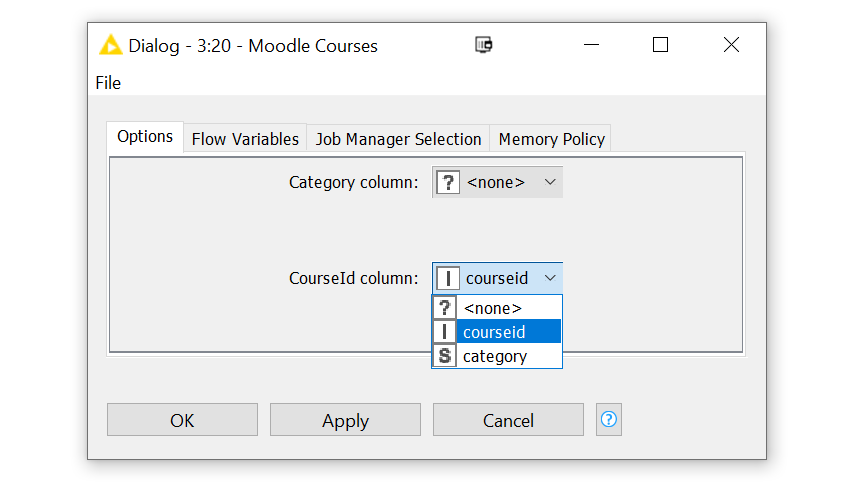
\includegraphics[width=1\textwidth]{img/nodes_moodle_courses_settings.png}
	\caption{Nodo \node{Moodle Courses}. Configuración.}
	\label{fig:moodlecourses_settings}
\end{figure}
\FloatBarrier

En la tabla~\ref{tab:moodle_courses_desc} se muestra la estructura de los datos devueltos por cada curso encontrado en la plataforma Moodle: 

\begin{table}[!h]
	\begin{center}
		\begin{tabular}{p{0.3\textwidth}p{0.1\textwidth}p{0.6\textwidth}}
			\toprule
			\textbf{Columna} & \textbf{Tipo} & \textbf{Descripción}\\
			\otoprule
			\textbf{courseid} & integer & ID del curso \\
         \hline
			\textbf{shortname} & string & Descripción corta del curso \\
         \hline
         \textbf{fullname} & string & Nombre completo del curso \\
         \hline
         \textbf{displayname} & string & Nombre del curso que se muestra en el aula \\
         \hline
         \textbf{enrolledusercount} & string & Número de alumnos registrados en el curso \\
         \hline
         \textbf{idnumber} & string & ID interno del curso \\
         \hline
         \textbf{visible} & boolean & Indica si el curso es visible para los estudiantes (1) \\
         \hline
         \textbf{summary} & string & Resumen o descripción del curso\\
         \hline
         \textbf{summaryformat} & boolean & Indica si el resumen tiene formato de texto asociado (1) \\
         \hline
         \textbf{format} & string & Tipo de formato del resumen \\
         \hline
         \textbf{category} & string & ID de categoría \\
         \hline
         \textbf{categoryname} & string & Nombre de la categoría \\
			\bottomrule
		\end{tabular}
	\end{center}
	\caption{Tabla de salida del nodo \node{Moodle Courses}.}
	\label{tab:moodle_courses_desc}
\end{table}
\FloatBarrier


\begin{figure}[!h]
	\centering
	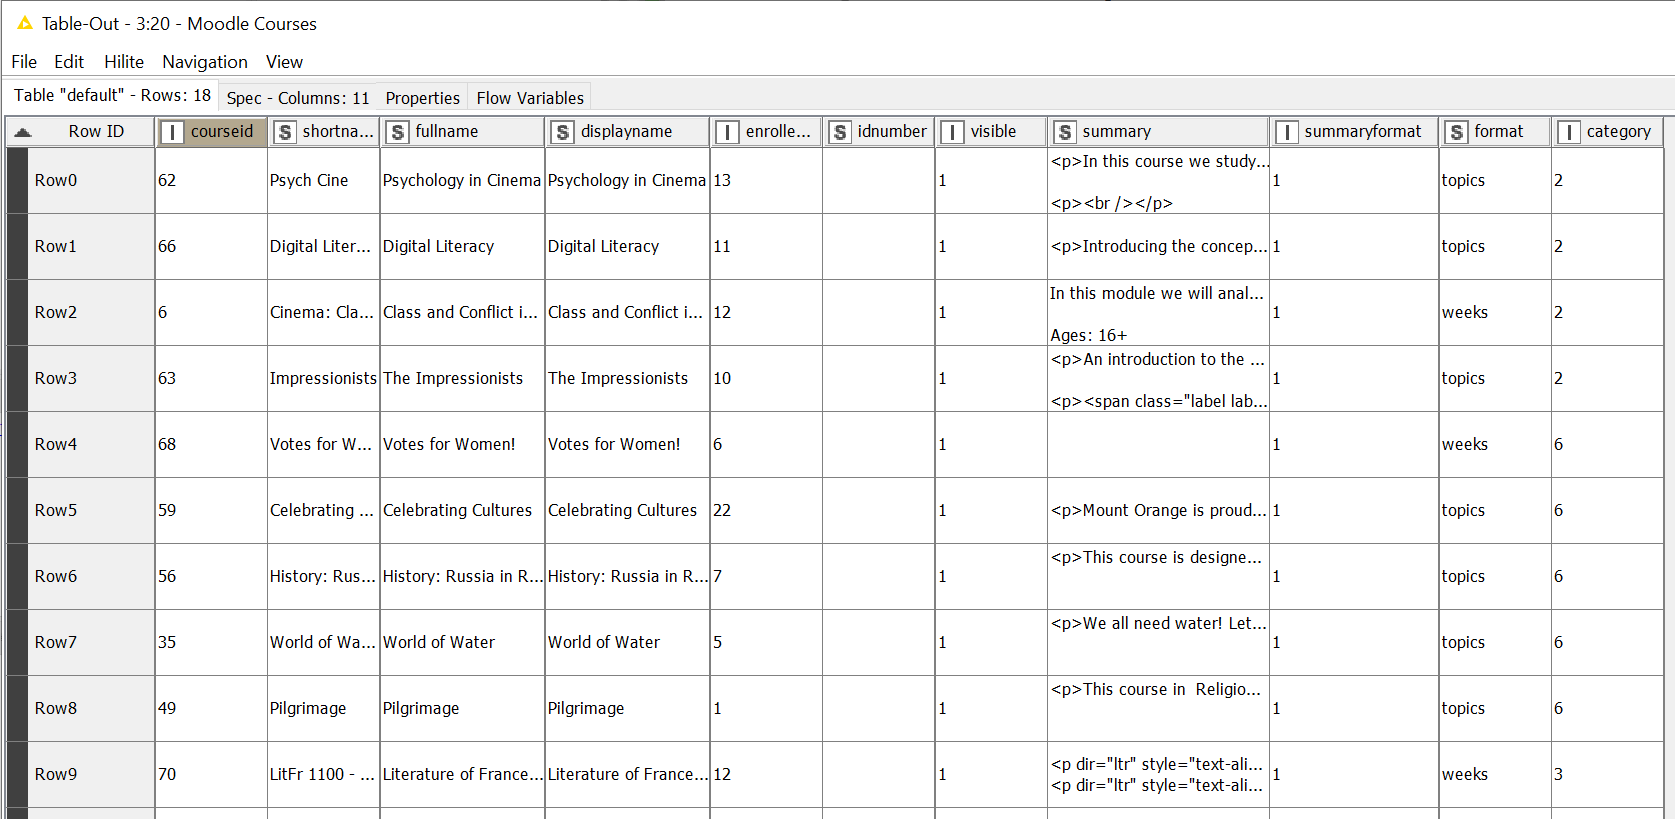
\includegraphics[width=1\textwidth]{img/nodes_moodle_courses_output.png}
	\caption{\node{Nodo Moodle Courses}. Ejemplo de salida.}
	\label{fig:moodlecourses_output}
\end{figure}
\FloatBarrier
\hphantom{ }


\newpage
\subsection{Diseño del nodo Moodle Users}

El nodo \node{Moodle Users} extrae información de usuarios según los cursos especificados (RF-3.1). 
También es posible devolver solo los usuarios con rol estudiante (RF-3.2), estimar el género de cada
usuario a partir de su nombre (RF-3.3) y anonimizar los datos personales (RF-3.4). 
\

El nodo tiene la siguiente \textbf{estructura}:

\begin{itemize}
	\item \textbf{Puertos de entrada}: 
    \begin{itemize}
		\item \textbf{0. Moodle Connection}. Conexión obtenida desde el nodo \node{Moodle Connector}. 
		\item \textbf{1. Input table}. Tabla de entrada con un listado de identificadores de cursos. 
   	\end{itemize}

	\item \textbf{Puertos de salida}: 
    \begin{itemize}
		\item \textbf{0. Moodle Connection}. Devuelve la conexión para facilitar su transferencia al siguiente nodo del flujo de trabajo. 
		\item \textbf{1. Output table}. Tabla de salida con la información de los usuarios. 
   	\end{itemize}

\end{itemize}


\begin{figure}[!h]
	\centering
	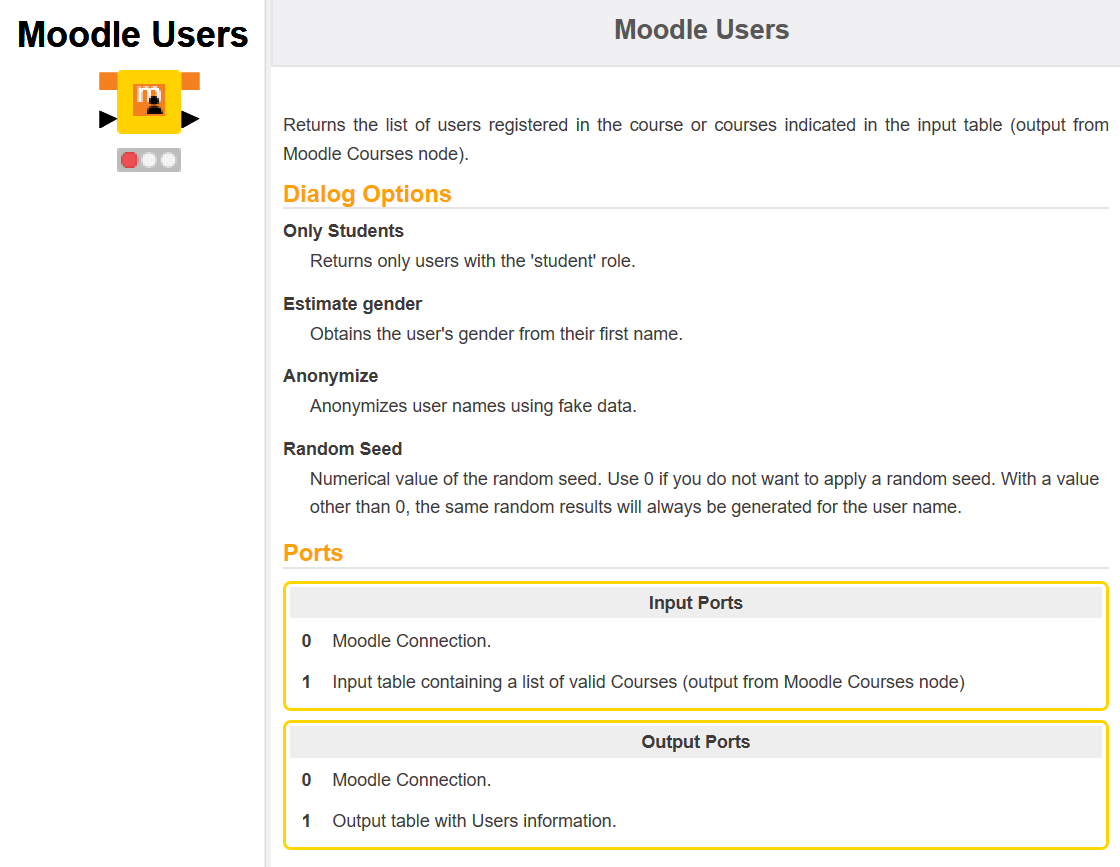
\includegraphics[width=1\textwidth]{img/nodes_moodle_users.png}
	\caption{Nodo \node{Moodle Users}. Descripción.}
	\label{fig:moodleusers}
\end{figure}
\FloatBarrier



El nodo permite la siguiente \textbf{configuración}: 

\begin{itemize}
   \item \textbf{Only students}. Si se activa, devuelve únicamente los usuarios con rol estudiante. 
   \item \textbf{Estimate gender}. Si se activa, devuelve una estimación del género del usuario (\english{male} o \english{female}). 
   \item \textbf{Anonymize}. Si se activa, devuelve el nombre y apellidos del usuario anonimizados.  
   \item \textbf{Random Seed}. Establece una semilla aleatoria para obtener un valor de nombre/apellidos anonimizado. 
   Si se deja el valor 0, los nombres/apellidos de cada usuario cambiarán con cada ejecución del nodo. 
\end{itemize}

\begin{figure}[!h]
	\centering
	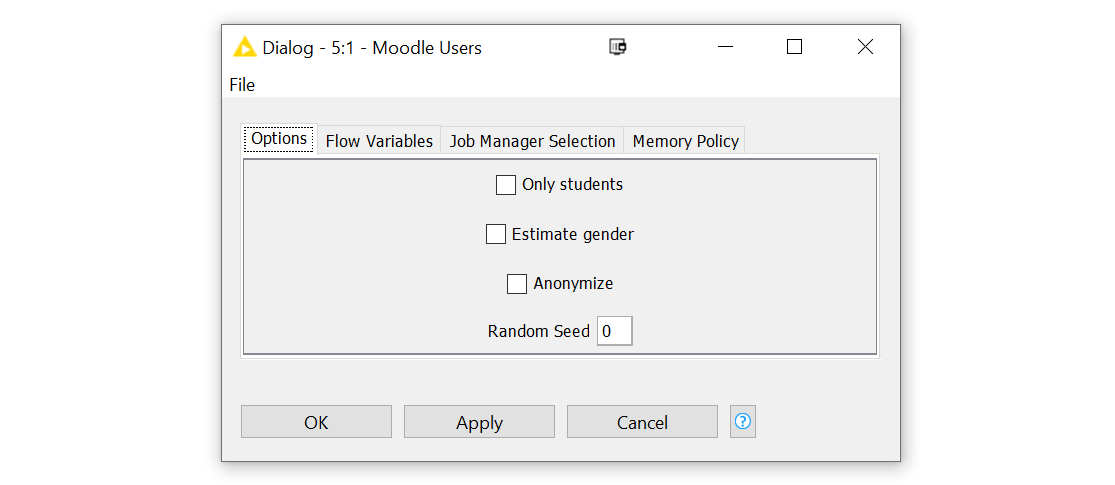
\includegraphics[width=1\textwidth]{img/nodes_moodle_users_settings.png}
	\caption{Nodo \node{Moodle Users}. Configuración.}
	\label{fig:moodleusers_settings}
\end{figure}
\FloatBarrier


En la tabla~\ref{tab:moodle_users_desc} se muestra la estructura de los datos devueltos por cada usuario: 

\begin{table}[!h]
	\begin{center}
		\begin{tabular}{p{0.25\textwidth}p{0.15\textwidth}p{0.6\textwidth}}
			\toprule
			\textbf{Columna} & \textbf{Tipo} & \textbf{Descripción}\\
			\otoprule
			\textbf{courseid} & integer & ID del curso en que el usuario está registrado\\
         \hline
			\textbf{userid} & integer & ID del usuario \\
         \hline
         \textbf{fullname} & string & Nombre completo del usuario. Puede ser el nombre real o el nombre Anonimizado, si se especifica en la configuración del nodo. \\
         \hline
         \textbf{firstaccess} & timestamp & Fecha de primer acceso al curso \\
         \hline
         \textbf{lastcourseaccess} & timestamp &  Fecha de último acceso al curso\\
         \hline
         \textbf{lastaccess} & timestamp & Fecha de último acceso a la plataforma \\
         \hline
         \textbf{roles} & string & Listado de roles del usuario, separados por coma \\
         \hline
         \textbf{country} & string & Código del país del usuario \\
         \hline
         \textbf{city} & string & Ciudad del usuario \\
         \hline
         \textbf{gender} & string & Género estimado (\english{male}, \english{female}). Esta columna es opcional, en función de la configuración del nodo. \\
			\bottomrule
		\end{tabular}
	\end{center}
	\caption{Tabla de salida del nodo \node{Moodle Users}.}
	\label{tab:moodle_users_desc}
\end{table}
\FloatBarrier

\begin{figure}[!h]
	\centering
	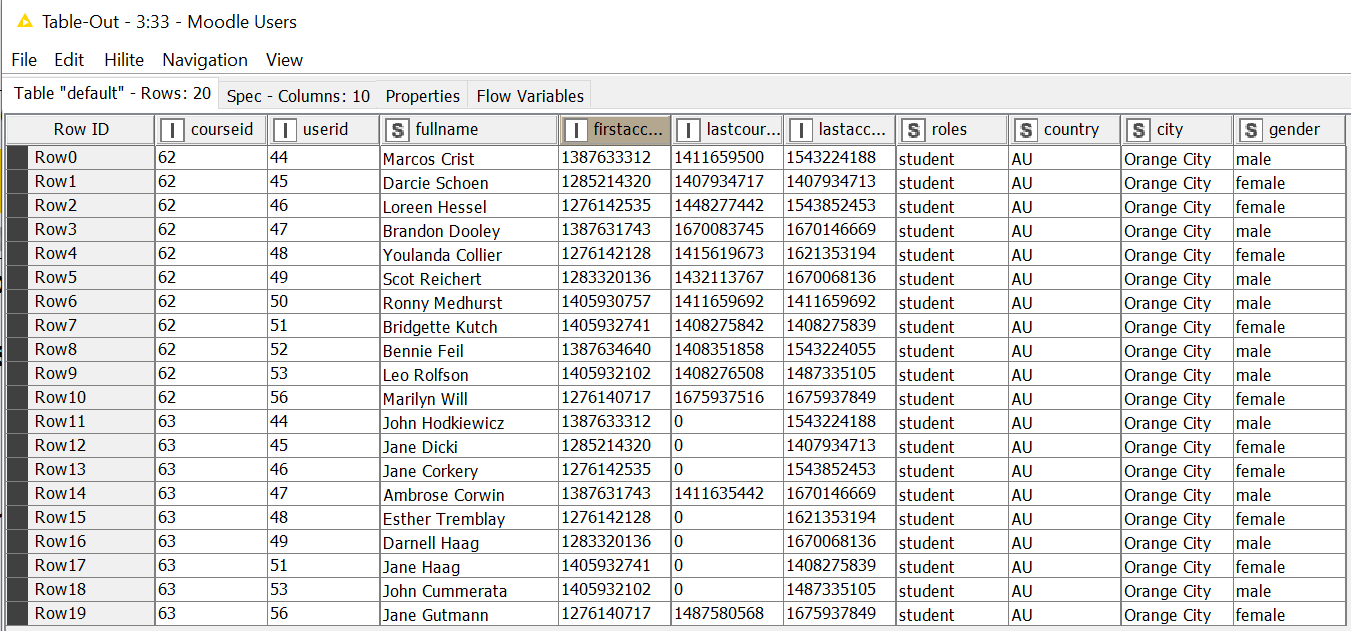
\includegraphics[width=1\textwidth]{img/nodes_moodle_users_output.png}
	\caption{Nodo \node{Moodle Users}. Salida de ejemplo. }
	\label{fig:moodleusers_output}
\end{figure}
\FloatBarrier
\hphantom{ }

\newpage
\subsection{Diseño del nodo Moodle Reports Logs}

El nodo \node{Moodle Reports Logs} extrae información de \english{logs} de la plataforma Moodle (RF-4). 
Este nodo está diseñado para poder extraer logs de forma homogénea aunque provengan de diferentes
fuentes dentro de Moodle (\english{Logs, Live logs, Activity Reports, Overview Statistics, Course Participation, Activity completion, Statistics, etc.})

\

El nodo tiene la siguiente \textbf{estructura}:

\begin{itemize}
	\item \textbf{Puertos de entrada}: 
    \begin{itemize}
		\item \textbf{0. Moodle Connection}. Conexión obtenida desde el nodo \node{Moodle Connector}. 
		\item \textbf{1. Input table}. Tabla de entrada con un listado de identificadores de cursos. 
   	\end{itemize}

	\item \textbf{Puertos de salida}: 
    \begin{itemize}
		\item \textbf{0. Moodle Connection}. Devuelve la conexión para facilitar su transferencia al siguiente nodo del flujo de trabajo. 
		\item \textbf{1. Output table}. Tabla de salida con la información de los \english{logs} o eventos. 
   	\end{itemize}

\end{itemize}

\begin{figure}[!h]
	\centering
	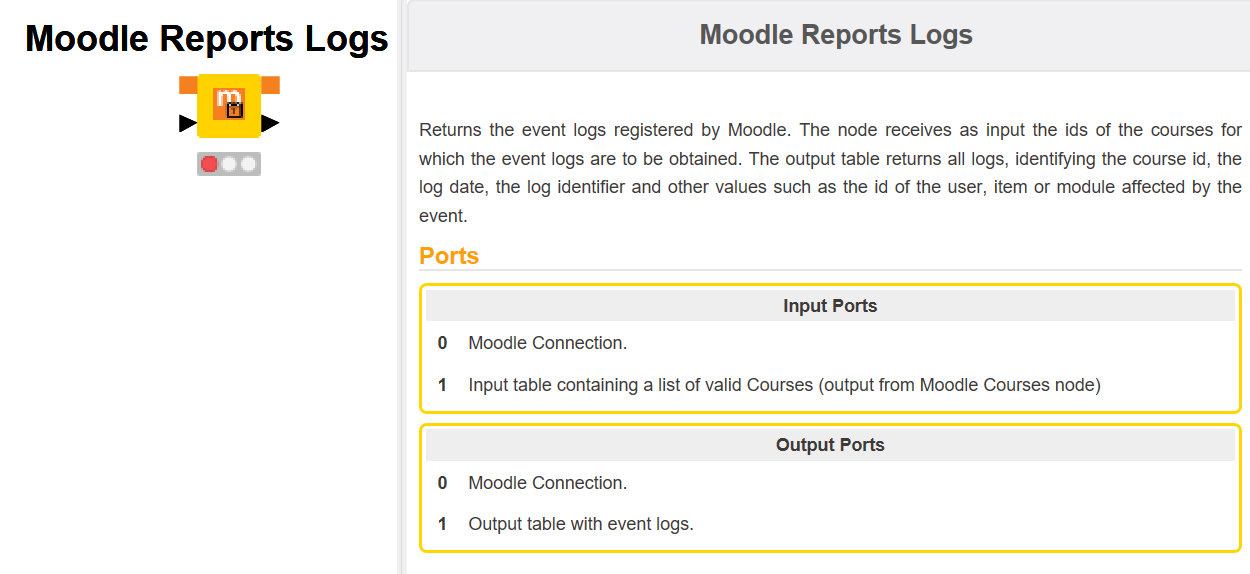
\includegraphics[width=1\textwidth]{img/nodes_moodle_reports_logs.png}
	\caption{Nodo \node{Moodle Reports Logs}. Descripción.}
	\label{fig:moodlereportslogs}
\end{figure}
\FloatBarrier

El nodo no tiene configuración específica. 
\

En la tabla~\ref{tab:moodle_reports_logs_desc} se muestra la estructura de los datos devueltos por cada evento del \english{log}: 

\begin{table}[!h]
	\begin{center}
		\begin{tabular}{p{0.3\textwidth}p{0.1\textwidth}p{0.6\textwidth}}
			\toprule
			\textbf{Columna} & \textbf{Tipo} & \textbf{Descripción}\\
			\otoprule
			\textbf{courseid} & integer & ID del curso \\
         \hline
			\textbf{time} & string & Fecha de registro del log en formato DD/MM/YYYY - HH:MM:SS +TimeZone. \\
         \hline
         \textbf{component} & string & Nombre del componente o módulo de Moodle que registra el evento \\
         \hline
         \textbf{eventName} & string & Nombre de sistema del evento \\
         \hline
         \textbf{origin} & string & Origen (WEB, CLI, APP, etc.) \\
         \hline
         \textbf{IPAddress} & string & Dirección IP del usuario \\
         \hline
         \textbf{course} & string & ID del curso extraído del mensaje de log \\
         \hline
         \textbf{user} & string & ID del usuario extraído del mensaje de log \\
         \hline
         \textbf{targetUser} & string & ID del usuario objetivo extraído del mensaje de log \\
         \hline
         \textbf{targetCourse} & string &  ID del curso objetivo extraído del mensaje de log \\
         \hline
         \textbf{module} & string &  ID del módulo extraído del mensaje de log \\
         \hline
         \textbf{section} & string &  ID de la sección extraído del mensaje de log \\
         \hline
         \textbf{item} & string &  ID del ítem extraído del mensaje de log \\
         \hline
         \textbf{description} & string & Mensaje completo guardado en el log \\
         \hline
         \textbf{descriptionMapped} & boolean &  Indica si el mensaje ha sido mapeado (1) o no (0)\\
         \hline
         \textbf{label} & string & Nombre del módulo (página, cuestionario, tarea, etc.) \\
         \bottomrule
		\end{tabular}
	\end{center}
	\caption{Tabla de salida del nodo \node{Moodle Reports Logs}.}
	\label{tab:moodle_reports_logs_desc}
\end{table}
\FloatBarrier

\begin{figure}[!h]
	\centering
	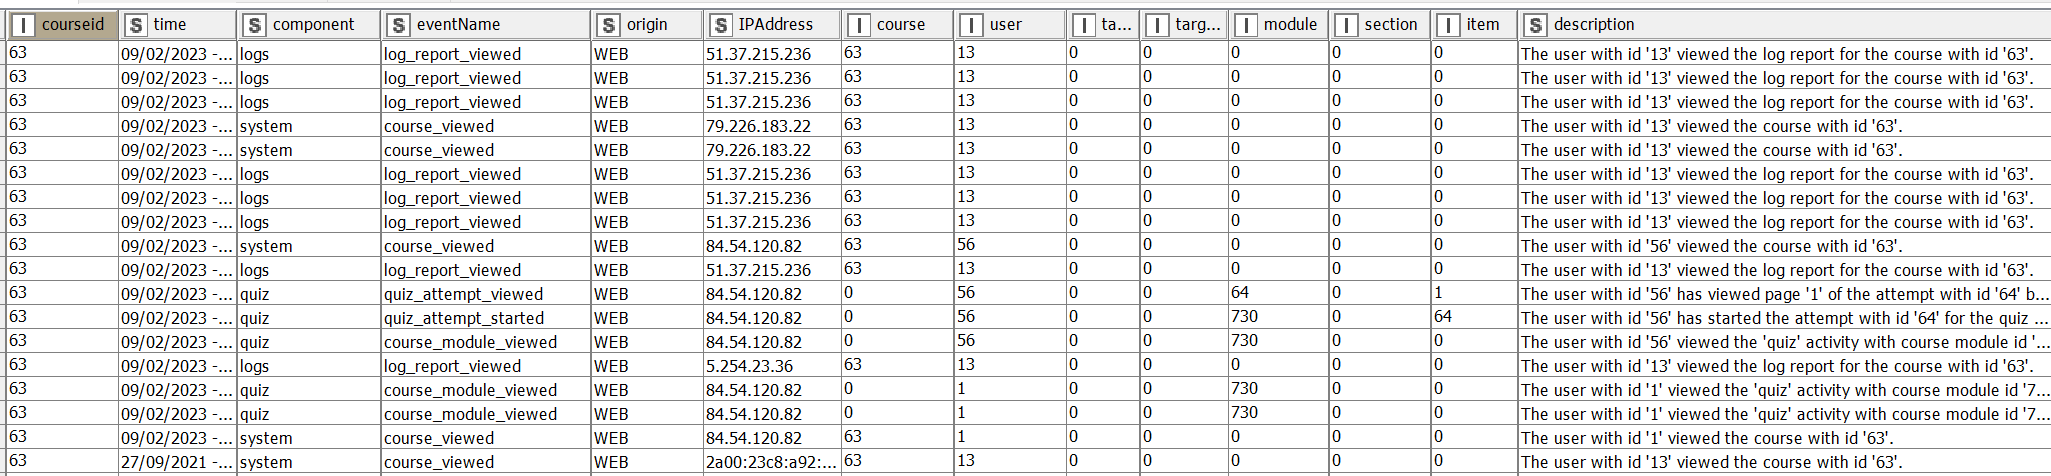
\includegraphics[width=1\textwidth]{img/nodes_moodle_reports_logs_output.png}
	\caption{Nodo \node{Moodle Reports Logs}. Salida.}
	\label{fig:moodlereportslogs_output}
\end{figure}
\FloatBarrier
\hphantom{ }




\newpage
\subsection{Diseño del nodo Moodle Reports Grades}

El nodo \node{Moodle Reports Grades} extrae información de calificaciones agrupadas por curso, estudiante y actividad (RF-5). Adicionalmente, devuelve una columna con la calificación final obtenida. 
\

El nodo tiene la siguiente \textbf{estructura}:

\begin{itemize}
	\item \textbf{Puertos de entrada}: 
    \begin{itemize}
		\item \textbf{0. Moodle Connection}. Conexión obtenida desde el nodo \node{Moodle Connector}. 
		\item \textbf{1. Input table}. Tabla de entrada con un listado de identificadores de cursos. 
   	\end{itemize}

	\item \textbf{Puertos de salida}: 
    \begin{itemize}
		\item \textbf{0. Moodle Connection}. Devuelve la conexión para facilitar su transferencia al siguiente nodo del flujo de trabajo. 
		\item \textbf{1. Output table}. Tabla de salida con la información de calificaciones. 
   	\end{itemize}

\end{itemize}

\begin{figure}[!h]
	\centering
	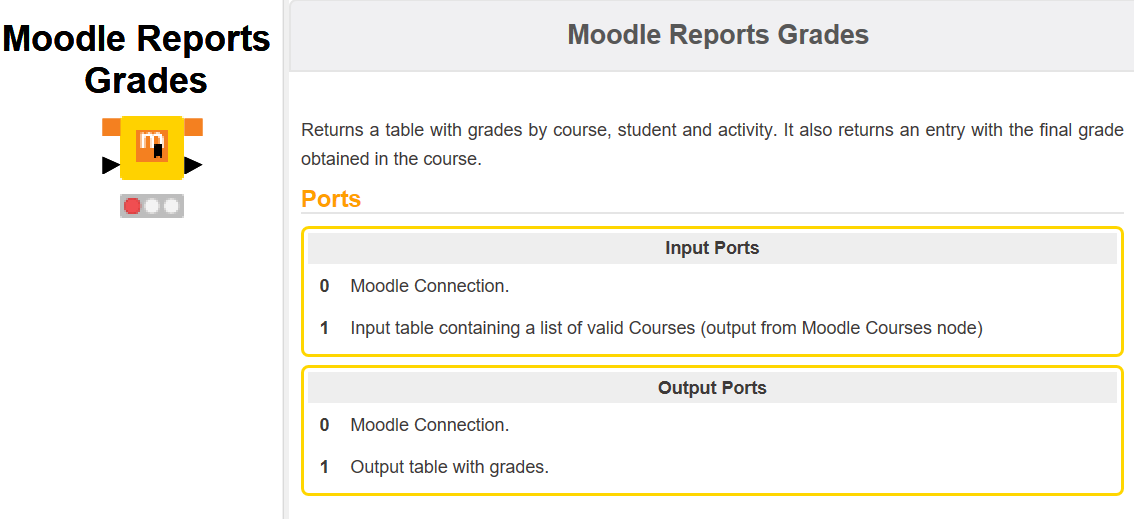
\includegraphics[width=1\textwidth]{img/nodes_moodle_reports_grades.png}
	\caption{Nodo \node{Moodle Reports Grades}. Descripción.}
	\label{fig:moodlereportsgrades}
\end{figure}
\FloatBarrier

El nodo no tiene configuración específica. 
\

En la tabla~\ref{tab:moodle_reports_grades_desc} se muestra la estructura de los datos devueltos por cada calificación, clasificada por curso/actividad/usuario: 

\begin{table}[!h]
	\begin{center}
		\begin{tabular}{p{0.25\textwidth}p{0.15\textwidth}p{0.6\textwidth}}
			\toprule
			\textbf{Columna} & \textbf{Tipo} & \textbf{Descripción}\\
			\otoprule
			\textbf{courseid} & integer & ID del curso en que está registrado el usuario \\
         \hline
			\textbf{userid} & integer & ID del usuario \\
         \hline
         \textbf{gradeid} & integer & ID de la calificación \\
         \hline
         \textbf{gradename} & string & Nombre de la actividad de calificación \\
         \hline
         \textbf{gradetype} & string & Tipo de calificación (mod, category, manual, course) \\
         \hline
         \textbf{grademodule} & string & Módulo de la actividad de calificación (assign, forum, quiz, etc.) \\
         \hline
         \textbf{grademin} & double & Valor mínimo de la calificación \\
         \hline
         \textbf{grademax} & double & Valor máximo de la calificación \\
         \hline
         \textbf{graderaw} & double & Calificación obtenida, sin formatear/procesar \\
         \hline
         \textbf{gradeformatted} & string & Calificación formateada \\
         \hline
         \textbf{gradecategoryid} & integer & ID de categoría de calificación \\
         \bottomrule
		\end{tabular}
	\end{center}
	\caption{Tabla de salida del nodo \node{Moodle Reports Grades}.}
	\label{tab:moodle_reports_grades_desc}
\end{table}
\FloatBarrier

\begin{figure}[!h]
	\centering
	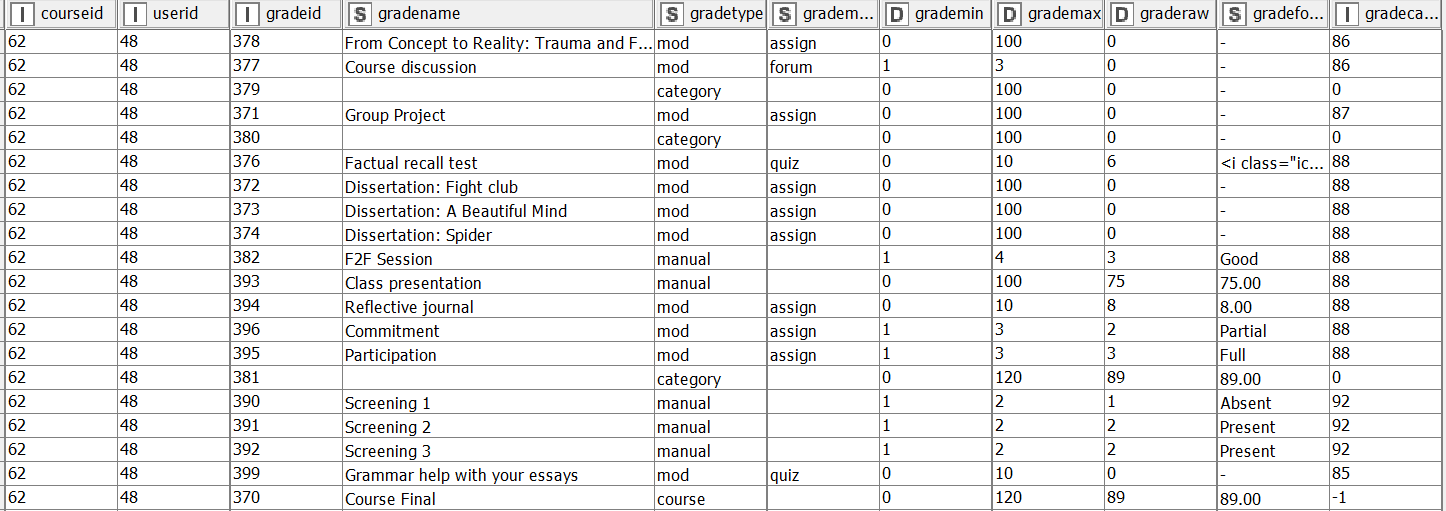
\includegraphics[width=1\textwidth]{img/nodes_moodle_reports_grades_output.png}
	\caption{Nodo \node{Moodle Reports Grades}. Salida.}
	\label{fig:moodlereportsgrades_output}
\end{figure}
\FloatBarrier
\hphantom{ }


\newpage
\subsection{Diseño del nodo Moodle Reports Quizzes}

El nodo \node{Moodle Reports Quizzes} extrae información sobre los intentos realizados por los estudiantes en los cuestionarios (RF-6). 
\

El nodo tiene la siguiente \textbf{estructura}:

\begin{itemize}
	\item \textbf{Puertos de entrada}: 
    \begin{itemize}
		\item \textbf{0. Moodle Connection}. Conexión obtenida desde el nodo \node{Moodle Connector}. 
		\item \textbf{1. Input table}. Tabla de entrada con un listado de identificadores de cursos. 
   	\end{itemize}

	\item \textbf{Puertos de salida}: 
    \begin{itemize}
		\item \textbf{0. Moodle Connection}. Devuelve la conexión para facilitar su transferencia al siguiente nodo del flujo de trabajo. 
		\item \textbf{1. Output table}. Tabla de salida con la información sobre los intentos realizados en cuestionarios. 
   	\end{itemize}

\end{itemize}


\begin{figure}[!h]
	\centering
	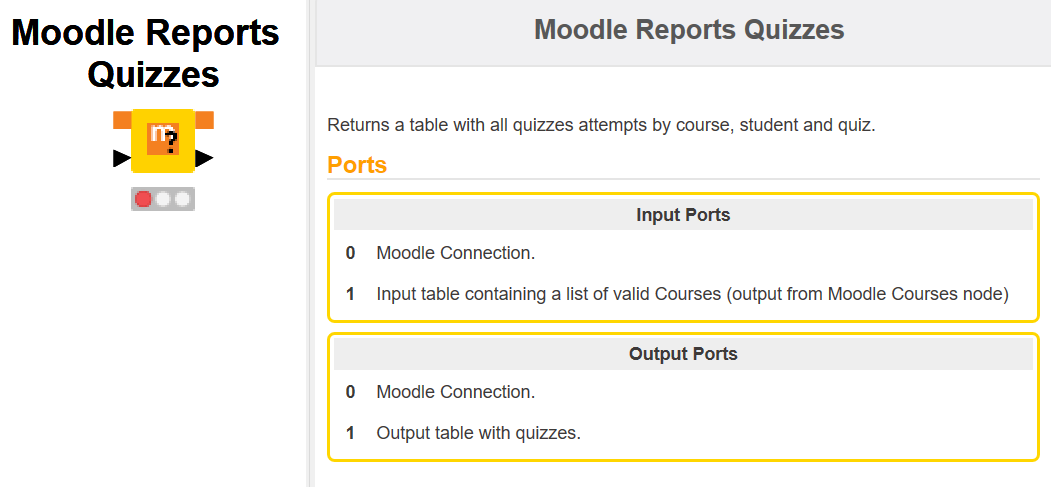
\includegraphics[width=1\textwidth]{img/nodes_moodle_reports_quizzes.png}
	\caption{Nodo \node{Moodle Reports Quizzes}. Descripción.}
	\label{fig:moodlereportsquizzes}
\end{figure}
\FloatBarrier


El nodo no tiene configuración específica. 
\

En la tabla~\ref{tab:moodle_reports_quizzes_desc} se muestra la estructura de los datos devueltos por cada intento de realización de cuestionario: 

\begin{table}[!h]
	\begin{center}
		\begin{tabular}{p{0.25\textwidth}p{0.15\textwidth}p{0.6\textwidth}}
			\toprule
			\textbf{Columna} & \textbf{Tipo} & \textbf{Descripción}\\
			\otoprule
			\textbf{courseid} & integer & ID del curso en que está registrado el usuario \\
         \hline
			\textbf{userid} & integer & ID del usuario \\
         \hline
         \textbf{coursemoduleid} & integer & ID del módulo \\
         \hline
		 \textbf{quizid} & integer & ID del cuestionario \\
         \hline
         \textbf{quizname} & string & Nombre del cuestionario \\
         \hline
		 \textbf{attemptid} & integer & ID del intento de resolución del cuestionario \\
         \hline
		 \textbf{attemptnumber} & integer & Número del intento de resolución del cuestionario \\
         \hline
		 \textbf{attemptduration} & integer & Duración del intento en segundos \\
         \hline
         \textbf{attemptgrade} & double & Calificación obtenida en este intento \\
         \bottomrule
		\end{tabular}
	\end{center}
	\caption{Tabla de salida del nodo \node{Moodle Reports Quizzes}.}
	\label{tab:moodle_reports_quizzes_desc}
\end{table}
\FloatBarrier


\begin{figure}[!h]
	\centering
	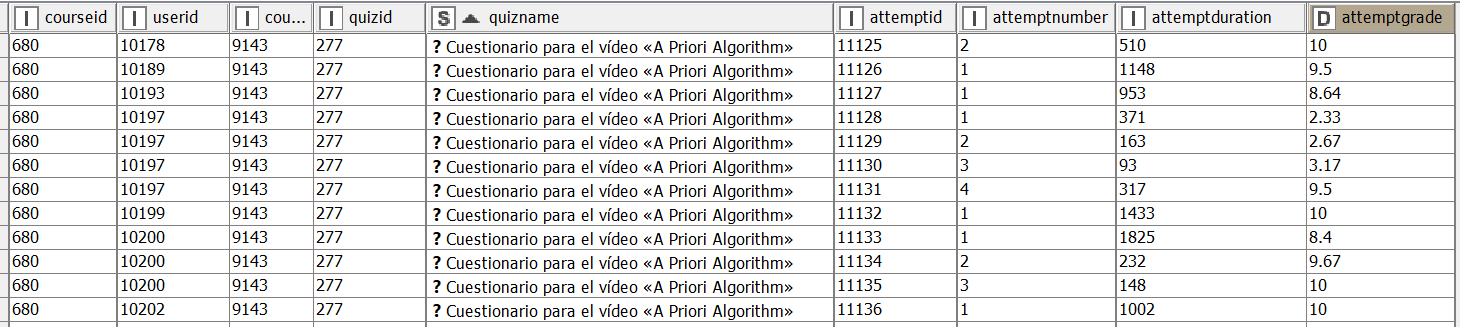
\includegraphics[width=1\textwidth]{img/nodes_moodle_reports_quizzes_output.png}
	\caption{Nodo \node{Moodle Reports Quizzes}. Salida.}
	\label{fig:moodlereportsquizzes_output}
\end{figure}
\FloatBarrier
\hphantom{ }



\apendice{Documentación técnica de programación}
\label{sec:appendixD}

\section{Introducción}

En este apéndice se describen los aspectos relevantes a nivel de programación para cualquier 
desarrollador interesado en continuar el proyecto o en desarrollar nuevas extensiones para la 
plataforma KNIME. 
\

\section{Estructura de directorios}

A continuación se presenta la estructura principal de archivos y carpetas de la extensión 
knime-moodle-integration desarrollada. No se han incluido las carpetas genéricas de definición 
del proyecto en Eclipse, que se pueden consultar directamente en el repositorio del proyecto. 

\begin{verbatim} 
\libraries -- Librerías externas (jar)
\src.org.knime.moodle.
  .internal  -- Librerías de uso interno
    .connection  -- Librería de conexión utilizada por el nodo Moodle Connector
      MoodleConnection.java
      MoodleConnectionPortObject.java
      MoodleConnectionPortObjectSpec.java
      MoodleLogin.Java
    .logs  -- Librería de Logs utilizada por el nodo Moodle Reports Logs
      Component.Java
      Component.java
      ComponentEvent.java
      Event.java
      LogDescription.java
      LogLine.java
      LogParameters.java
      Logs.java
      MoodleLogCreator.java
  .nodes  -- Nodos de la extensión
    .connector  -- Implementación del nodo Moodle Connector
      MoodleConnectorConfiguration.java
      MoodleConnectorNodeDialog.java
      MoodleConnectorNodeFactory.java
      MoodleConnectorNodeFactory.xml
      MoodleConnectorNodeModel.java
      MoodleConnectorNodePlugin.java
      MoodleConnectorNodeSettingsModel.java
      MoodleConnectorNodeView.java
      default.png
      moodle-connector.png
      package.html
    .courses  -- Implementación del nodo Moodle Courses
      MoodleCoursesNodeDialog.java
      MoodleCoursesNodeFactory.java
      MoodleCoursesNodeFactory.xml
      MoodleCoursesNodeModel.java
      MoodleCoursesNodeView.java
      default.png
      moodle-courses.png
      package.html
    .reports
      .grades  -- Implementación del nodo Moodle Reports Grades
        MoodleReportsGradesNodeDialog.java
        MoodleReportsGradesNodeFactory.java
        MoodleReportsGradesNodeFactory.xml
        MoodleReportsGradesNodeModel.java
        MoodleReportsGradesNodeView.java
        moodle-reports-grades.png
        package.html
      .logs  -- Implementación del nodo Moodle Reports Logs
        MoodleReportsLogsNodeDialog.java
        MoodleReportsLogsNodeFactory.java
        MoodleReportsLogsNodeFactory.xml
        MoodleReportsLogsNodeModel.java
        MoodleReportsLogsNodeView.java
        moodle-reports-logs.png
        package.html
    .users  -- Implementación del nodo Moodle Users
      MoodleUsersNodeDialog.java
      MoodleUsersNodeFactory.java
      MoodleUsersNodeFactory.xml
      MoodleUsersNodeModel.java
      MoodleUsersNodeView.java
      moodle-users.png
      package.html
\end{verbatim}



\subsection{Entorno de desarrollo con Eclipse y KNIME SDK}

Los nodos de KNIME se desarrollan en Java utilizando el IDE de programación Eclipse. Aunque desde la versión 4.6 también se permite
 la implementación de nodos totalmente programados en Python, en este proyecto los nodos se han implementado en Java para la versión KNIME 4.7.x. 
\

La documentación oficial de KNIME nos detalla paso a paso cómo preparar el entorno de trabajo necesario para desarrollar
 nuevos nodos en Java. Como primer paso debemos instalar Eclipse como IDE de desarrollo y KNIME SDK que nos proporciona las herramientas 
 necesarias de desarrollo para compilar nuestra extensión y ejecutarla en KNIME. Se pueden consultar las instrucciones detalladas en este enlace \url{https://github.com/knime/knime-sdk-setup}. 
\

Los pasos que tendremos que seguir son:

\begin{enumerate}
	\item Instalación de Java 17 (OpenJDK 17). Esta versión puede variar para futuras versiones de KNIME. 
	\item Instalar Eclipse. Debemos instalar la versión <<Eclipse for RCP and RAP Developers 2022-06>>, que es la que se corresponde a KNIME 4.7.x. 
  Esta versión varía en función de la versión de KNIME en la que vayamos a trabajar. 
	\item Instalar Git. 
	\item Descargar KNIME SDK y configurar eclipse. Siguiendo las instrucciones correspondientes, indicaremos cuál es la plataforma objetivo activa, de forma 
  que Eclipse pueda ejecutar KNIME y desplegar la extensión desarrollada. 
  \item Ejecutar KNIME desde KNIME Analytics Platform.launch $\triangleright$ Run as $\triangleright$ KNIME Analytics Platform. 
\end{enumerate}  


\subsection{Instalación y compilación de la extensión KNIME Moodle Integration}

Por último, necesitamos incorporar la extensión \node{knime-moodle-integration} importando el proyecto desde el repositorio. 
\



\section{Desarrollo de nuevos nodos}

Las instrucciones previas nos sirven para montar un entorno de desarrollo para trabajar con la extensión desarrollada en este proyecto. Si se desea implementar una nueva extensión, 
se recomienda seguir las instrucciones que KNIME nos facilita mediante la \href{https://docs.knime.com/latest/analytics_platform_new_node_quickstart_guide/index.html\#_introduction}{implementación de un nodo de ejemplo}. 


\apendice{Documentación de usuario}
\label{sec:appendixE}

\section{Introducción}

En la sección anterior se ha descrito cómo instalar y configurar el entorno de desarrollo con Eclipse y KNIME SDK. Si solo se desea
utilizar la extensión desarrollada en un flujo de trabajo, sin ánimos de modificarla a nivel de código, podemos seguir las siguientes instrucciones
de instalación. 

\section{Instalación KNIME}

Como la extensión KNIME Moodle Integration se ha implementado en KNIME 4.7.7, instalaremos esta versión desde la sección \href{https://www.knime.com/download-previous-versions}{Previous Versions of KNIME}. 
KNIME está disponible para Windows, Linux y macOS.


\section{Instalación de la extensión Moodle KNIME Integration}

La extensión lista para ser utiliza en cualquier instalación de KNIME está disponible como pre-release en el repositorio del proyecto: 

\url{https://github.com/frankgil/knime-moodle/releases/tag/extension}

Para utilizar esta extensión, debemos ejecutar KNIME y crear un Sitio de actualización local 
(Local Update Site). Seguiremos estos pasos:
\

En primer lugar descargaremos y descomprimiremos en una carpeta local la extensión. 
\

Desde KNIME $\triangleright$ \english{Preferences} $\triangleright$ \english{Install/Update} $\triangleright$ \english{Available Software Sites} $\triangleright$ \english{Add}, añadiremos 
una ubicación local seleccionando la carpeta <<org.knime.moodle.update>>, tal y como se muestra en la Figura ~\ref{fig:usuario1}: 

\begin{figure}[!htb]
	\centering
	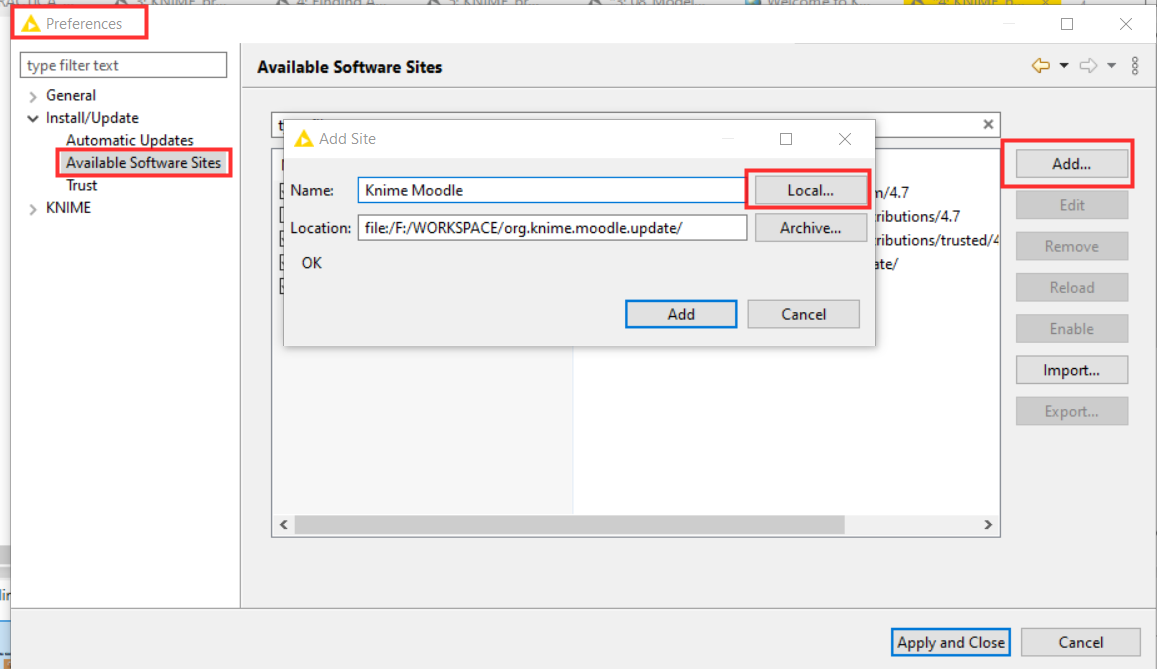
\includegraphics[width=1\textwidth]{img/manual_usuario_install_site_update1.png}
	\caption{Instalación de la extensión \node{Moodle} en KNIME 1.}
	\label{fig:usuario1}
\end{figure}
\FloatBarrier

A continuación seleccionamos el sitio añadido ~\ref{fig:usuario2},

\begin{figure}[!htb]
	\centering
	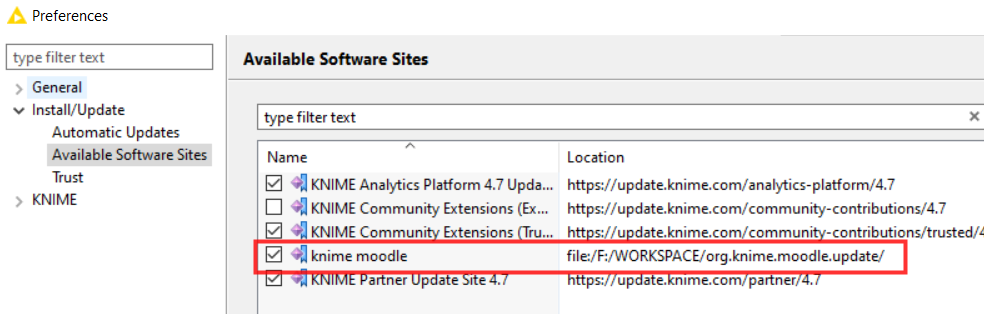
\includegraphics[width=1\textwidth]{img/manual_usuario_install_site_update2.png}
	\caption{Instalación de la extensión \node{Moodle} en KNIME 2.}
	\label{fig:usuario2}
\end{figure}
\FloatBarrier

y seleccionamos la instalación Moodle que queremos instalar ~\ref{fig:usuario3}.

\begin{figure}[!htb]
	\centering
	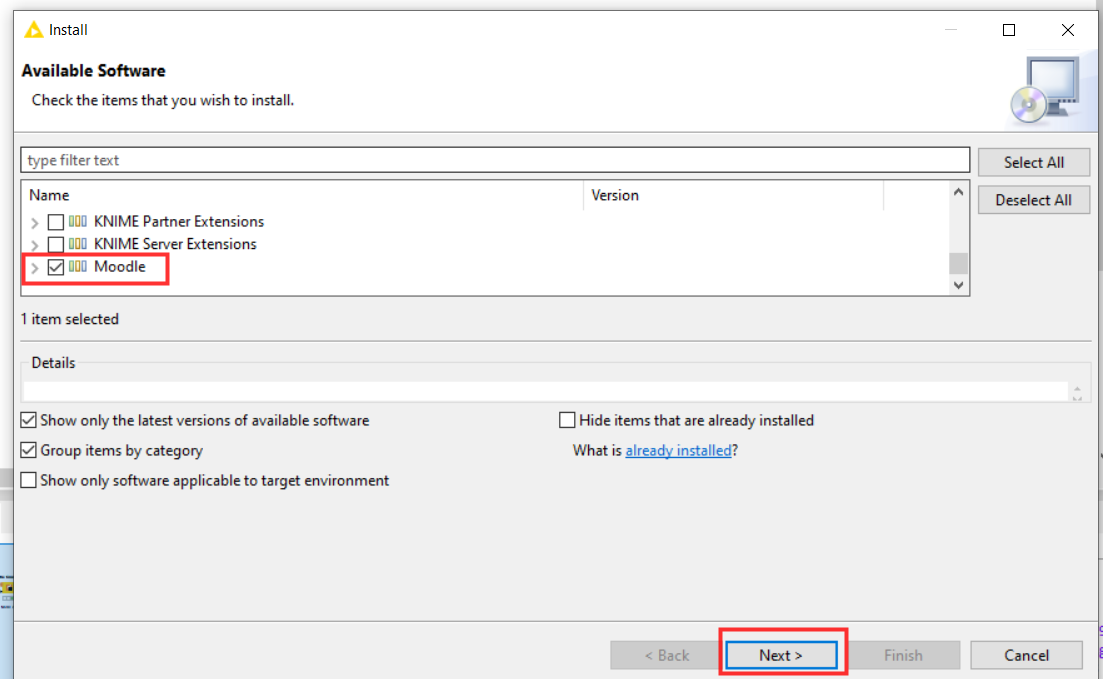
\includegraphics[width=1\textwidth]{img/manual_usuario_install_site_update3.png}
	\caption{Instalación de la extensión \node{Moodle} en KNIME 3.}
	\label{fig:usuario3}
\end{figure}
\FloatBarrier

Nos mostrará detalles de la extensión a instalar antes de completar la instalación ~\ref{fig:usuario4}. 

\begin{figure}[!htb]
	\centering
	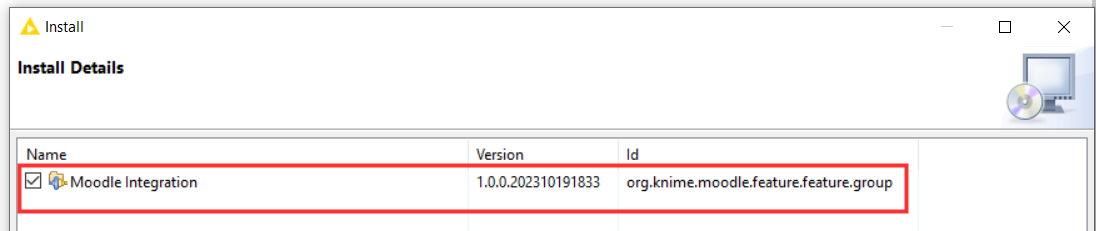
\includegraphics[width=1\textwidth]{img/manual_usuario_install_site_update4.png}
	\caption{Instalación de la extensión \node{Moodle} en KNIME 4.}
	\label{fig:usuario4}
\end{figure}
\FloatBarrier

Los nodos de la extensión \node{Moodle} se verán ahora en el repositorio de nodos ~\ref{fig:usuario5}. 

\begin{figure}[!htb]
	\centering
	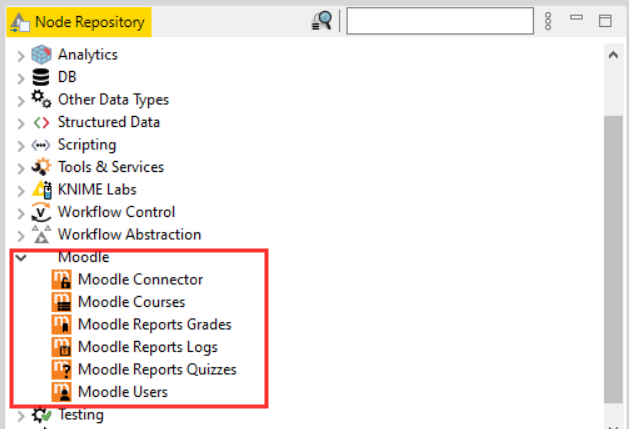
\includegraphics[width=1\textwidth]{img/manual_usuario_install_site_update5.png}
	\caption{Instalación de la extensión \node{Moodle} en KNIME 5.}
	\label{fig:usuario5}
\end{figure}
\FloatBarrier

\hphantom{ }

\newpage
\section{Crear un \english{workflow} y usar la extensión}

Ahora ya podremos crear \english{workflows} de KNIME incorporando los nodos de integración con Moodle y 
combinándolos con otros nodos de KNIME. Crea un nuevo Workflow desde \english{File} $\triangleright$ \english{New} $\triangleright$ \english{New KNIME Workflow} y sigue los siguientes pasos:  
\

Localiza en el repositorio de nodos el nodo \node{Moodle Connector} y añádelo al \english{Workflow} como se muestra en la Figura~\ref{fig:extension0}.

\begin{figure}[!htb]
	\centering
	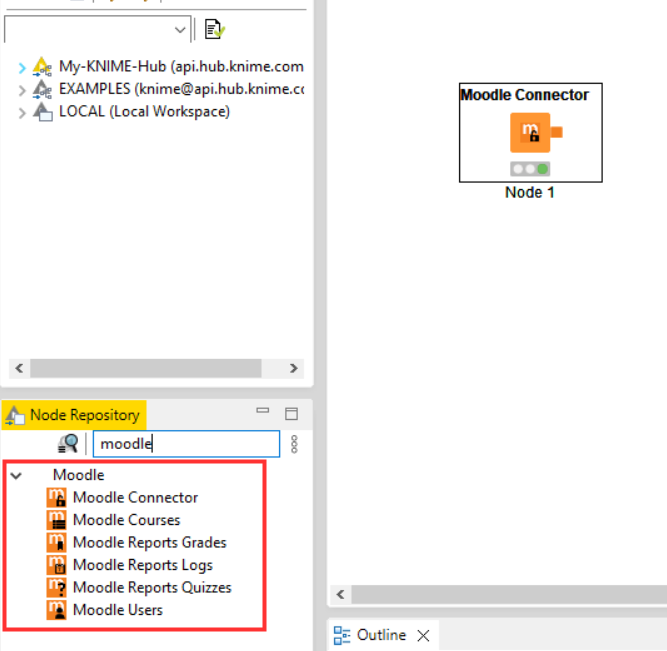
\includegraphics[width=1\textwidth]{img/manual_usuario_node_repository.png}
	\caption{Usando la extensión \node{Moodle}. Repositorio de nodos. }
	\label{fig:extension0}
\end{figure}
\FloatBarrier

Configura el nodo para conectar con una plataforma Moodle a la que tengas acceso ~\ref{fig:extension1}. 
\

\begin{figure}[!htb]
	\centering
	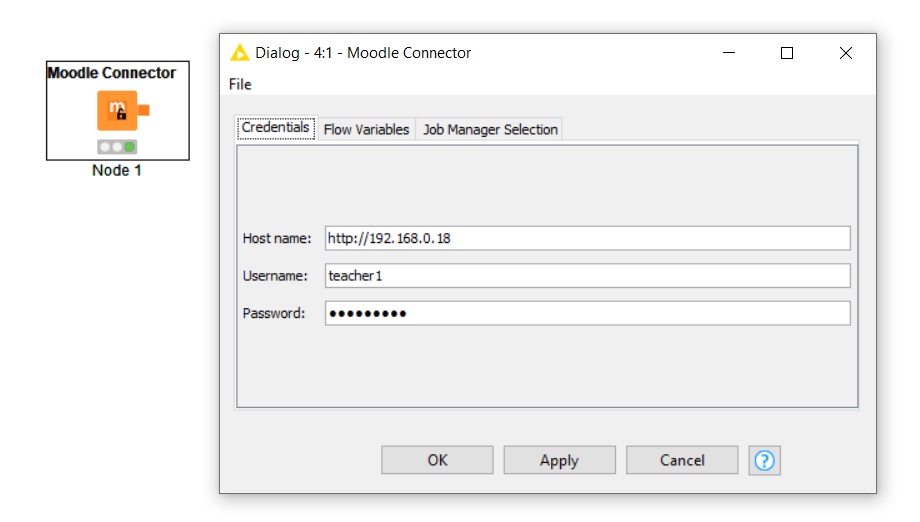
\includegraphics[width=1\textwidth]{img/manual_usuario_moodle_connector.png}
	\caption{Usando la extensión \node{Moodle} 1.}
	\label{fig:extension1}
\end{figure}
\FloatBarrier

Ejecuta el \english{workflow} y comprueba que se conecta correctamente a Moodle. En la información de 
depuración por Consola de KNIME~\ref{fig:extension2} verás las entradas \ruta{MoodleConnector} con 
información relativa al token de conexión, id del usuario y token del webservice. 
Si no recibes esta información, revisa que los datos de conexión en el nodo sean correctos. 
\

\begin{figure}[!htb]
	\centering
	\includegraphics[width=1\textwidth]{img/manual_usuario_moodle_connector_login.png}
	\caption{Usando la extensión \node{Moodle} 2.}
	\label{fig:extension2}
\end{figure}
\FloatBarrier

Añade a continuación un nodo de tipo \node{Moodle Courses}. El nodo necesita como entrada la salida de un nodo de tipo \node{Table Creator}. 
Une los nodos y configura la tabla con dos columnas, \field{category} y \field{courseid} ~\ref{fig:extension3}. En estas columnas podrás indicar 
los identificados de categorías o cursos de tu plataforma Moodle. Aunque el contenido de la tabla 
es optativo, debe añadirse y enlazarse el nodo correspondiente. 

\begin{figure}[!htb]
	\centering
	\includegraphics[width=1\textwidth]{img/manual_usuario_moodle_courses_table.png}
	\caption{Usando la extensión \node{Moodle} 3.}
	\label{fig:extension3}
\end{figure}
\FloatBarrier


En la configuración del nodo \node{Moodle Courses}, selecciona la columna 
correspondiente a la categoría y la correspondiente a los identificadores de cursos ~\ref{fig:extension4}. 

\begin{figure}[!htb]
	\centering
	\includegraphics[width=1\textwidth]{img/manual_usuario_moodle_courses_config.png}
	\caption{Usando la extensión \node{Moodle} 4.}
	\label{fig:extension4}
\end{figure}
\FloatBarrier

Por último, ejecuta el \english{workflow} y comprueba la tabla de salida de \node{Moodle Courses}. Debes obtener una 
salida como la mostrada en la Figura ~\ref{fig:extension5}, con información de los cursos.  

\begin{figure}[!htb]
	\centering
	\includegraphics[width=1\textwidth]{img/manual_usuario_moodle_courses_list.png}
	\caption{Usando la extensión \node{Moodle} 5.}
	\label{fig:extension5}
\end{figure}
\FloatBarrier

A partir de aquí puedes añadir el resto de nodos de la extensión y combinarlos con otros nodos de KNIME. 
Consulta el Apéndice \ref{sec:appendixC} para saber más el diseño y funcionalidad de los nodos disponibles en la extensión \node{KNIME Moodle Integration}. 


\bibliographystyle{plain}
\bibliography{bibliografia}

\end{document}
